
We investigate the fundamental limits of multiple testing problems in high-dimensional chi-square models, and in genome-wide association studies as introduced in Section \ref{sec:motivation-chisq}.

In Section \ref{sec:chisq-boundaries}, we shall establish the phase transitions of the sparse chi-square model \eqref{eq:model-chisq}.
Recall that in large-scale screening studies where a large number of association tests are conducted, resulting statistics may be approximated by
\begin{equation} \label{eq:model-chisq-Chapter6}
    %x(i) \distras{\mathrm{ind.}} \chi_\nu^2\left(\lambda(i)\right), \quad i=1,\ldots,p.
    x(i) \sim \chi_\nu^2\left(\lambda(i)\right), \quad i=1,\ldots,p,
\end{equation}
where $\chi_\nu^2\left(\lambda(i)\right)$ is a chi-square distributed random variable with $\nu$ degrees of freedom and non-centrality parameter $\lambda(i)$.
In parallel to results in Chapter \ref{chap:phase-transitions}, we show that several commonly used family-wise error rate-control procedures --- including Bonferroni's procedure --- are asymptotically optimal for the {exact}, and {exact-approximate} support recovery problems (as defined in Definition \ref{def:exact-recovery-success-failure}) in idealized chi-square models \eqref{eq:model-chisq-Chapter6} with independent components.
We further show that the \ac{BH} procedure is asymptotically optimal for the {approximate}, and {approximate-exact} support recovery problems.
% \ref{thm:chi-squared-exact-boundary}, \ref{thm:chi-squared-exact-approx-boundary}, \ref{thm:chi-squared-approx-boundary}, and \ref{thm:chi-squared-approx-exact-boundary}.
Under appropriate parametrizations of the signal sizes and sparsity, they establish the phase transitions of support recovery problems in the chi-square model.
Remarkably, the degree-of-freedom parameter does not affect the asymptotic boundaries in any of the four support recovery problems.

All phase transition boundaries coincide with those in the additive error models obtained in Chapter \ref{chap:phase-transitions} under suitable parametrizations.
% and Figure \ref{fig:phase-chi-squared} continues to apply.
indicating vanishing differences between the difficulties of the one-sided and two-sided alternatives in the Gaussian additive error model \eqref{eq:model-additive}.

\medskip

We then return to association screenings of categorical variables in
Section \ref{sec:odds-and-power}, and present the consequences of the phase transition in the exact-approximate problem in large-scale genetic association studies.
% present empirical evidence for the phase transition in the exact-approximate problem using real data from large-scale association studies on breast cancer obtained from the NHGRI-EBI GWAS Catalog \citep{macarthur2016new}.
% demystify the notion of signal size $\lambda$ in this context.
% which is perhaps less transparent than in additive error models.
We do so by characterizing the relationship between the signal size $\lambda$ and the marginal frequencies, odds ratio, and sample sizes for association tests on 2-by-2 contingency tables.
% Specifically, the amount of signal, when rare variants are present, is weaker compared to the signal when the marginal distributions are balanced.
% In other words, reliable detection of the effects by rare variants would require more samples compared to common variants, even at the same odds ratio.
This result, establishing the relationship between sample sizes and signal sizes, is made precise in Section \ref{sec:odds-and-power}.

We elaborate on the implications of this relationship on optimal study designs for association studies in Section \ref{sec:optimal-design}.
Perhaps surprisingly, our analysis reveals that balanced designs with equal number of cases and controls are often statistically inefficient.
Practical consequences of these results in power analysis will be illustrated with data examples in Section \ref{sec:phase-transitions-in-GWAS}. 

The phase transitions in the chi-square models are demonstrated with numerical simulations in Section \ref{sec:numerical}.
Proofs of results in this Chapter are collected in Section \ref{sec:proof-signal-size-odds-ratio}.

% Practical issues are also addressed to make for simple and effective power analysis.

\section{Support recovery problems in chi-squared models}
\label{sec:chisq-boundaries}

Similar to the analysis of additive error models in Chapter \ref{chap:phase-transitions}, we will work with triangular arrays of chi-square models \eqref{eq:model-chisq-Chapter6} indexed by $p$.
We adopt the same parametrization for the sparsity of the non-centrality parameter vectors $\lambda = \lambda_p$,
\begin{equation} \label{eq:signal-sparsity}
    |S_p| = \left\lfloor p^{1-\beta} \right\rfloor, \quad \beta\in(0,1]
\end{equation}
where $\beta$ parametrizes the problem sparsity.
The closer $\beta$ is to 1, the sparser the support $S_p$; conversely, when $\beta$ is close to 0, the support is dense with many non-null signals.

We parametrize the range of the non-zero and perhaps unequal signals in the chi-square model with
\begin{equation} \label{eq:signal-size}
    \underline{\Delta} = 2\underline{r}\log{p}
    \le \lambda(i) \le
    \overline{\Delta} = 2\overline{r}\log{p}, \quad \text{for all}\;\;i\in S_p,
\end{equation}
for some constants $0<\underline{r}\le\overline{r}\le+\infty$.

\subsection{The exact support recovery problem}
\label{subsec:exact-support-recovery-chisq}

The first main result characterizes the phase transition phenomenon in the exact support recovery problem under the chi-square model.

\begin{theorem} \label{thm:chi-squared-exact-boundary}
Consider the high-dimensional chi-squared model \eqref{eq:model-chisq-Chapter6} with signal sparsity and size as described in \eqref{eq:signal-sparsity} and \eqref{eq:signal-size}.
The function 
\begin{equation} \label{eq:exact-boundary-chisquared}
    g(\beta) = \left(1 + \sqrt{1-\beta}\right)^2
\end{equation}
characterizes the phase transition of exact support recovery problem.
Specifically, if $\underline{r} > {{g}}(\beta)$, then Bonferroni's, Sid\'ak's, Holm's, and Hochberg's procedures with slowly vanishing (see Definition \ref{def:slowly-vanishing}) nominal FWER levels all achieve asymptotically exact support recovery in the sense of \eqref{eq:support-recovery-success}. 

Conversely, if $\overline{r} < {{g}}(\beta)$, then for any thresholding procedure $\widehat{S}_p$, we have $\P[\widehat{S}_p=S_p]\to0$.
Therefore, in view of Lemma \ref{lemma:risk-exact-recovery-probability}, exact support recovery asymptotically fails for all thresholding procedures in the sense of \eqref{eq:support-recovery-failure}.
\end{theorem}

% \begin{figure}
%   \begin{center}
%     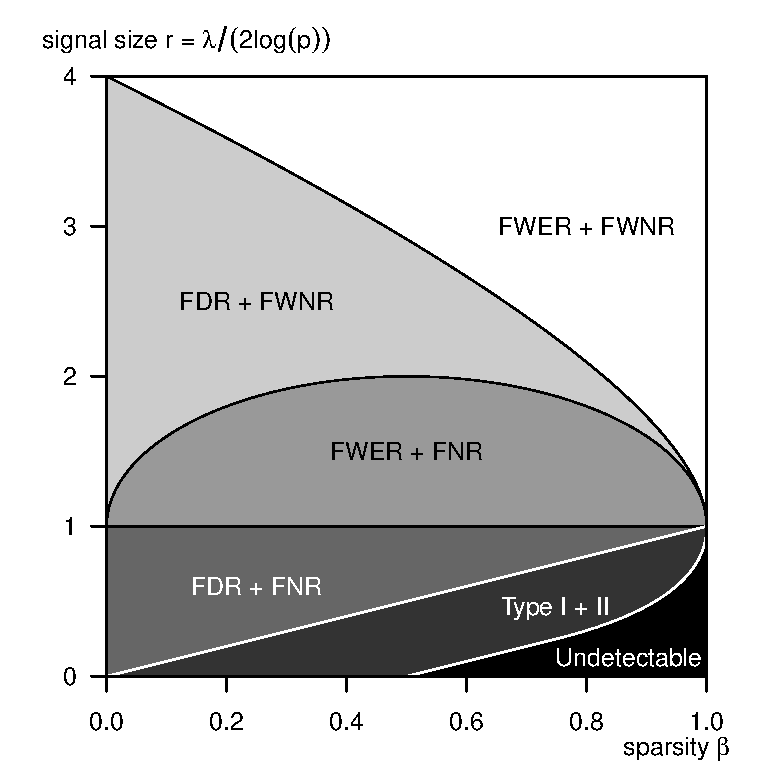
\includegraphics[width=0.7\textwidth]{./pics/phase_diagram_chisquared_ALL_boundaries.eps}
%   \end{center}
%    \caption{The phase diagram for the high-dimensional chi-square model \eqref{eq:model-chisq}, illustrating the boundaries of the exact support recovery (FWER + FWNR; top curve; Theorem \ref{thm:chi-squared-exact-boundary}), the approximate-exact support recovery (FDR + FWNR; second curve from top; Theorem \ref{thm:chi-squared-approx-exact-boundary}), the exact-approximate support recovery (FWER + FNR; horizontal line $r=1$; Theorem \ref{thm:chi-squared-exact-approx-boundary}), and the approximate support recovery problems (FDR + FNR; tilted line $r=\beta$; Theorem \ref{thm:chi-squared-approx-boundary}). The signal detection problem (type I + type II errors of the global test; lower curve) was studied in Donoho and Jin (2004). In each region of the diagram and above, the annotated statistical risk can be made to vanish, as dimension $p$ diverges. Conversely, the risks has liminf at least one. All boundaries are unaffected by the degree-of-freedom. All boundaries are identical to those in the Gaussian additive error model \eqref{eq:model-additive} under one-side alternatives; c.f., results in Section \ref{sec:additive-error-model-boundaries}.}
%    \label{fig:phase-chi-squared}
% \end{figure}


The procedures listed in Theorem \ref{thm:chi-squared-exact-boundary} were reviewed in Section \ref{sec:statistical-procedures}. 
Proof of the theorem can be found in Section \ref{subsec:proof-chi-squared-exact-boundary}. 
% The boundary \eqref{eq:exact-boundary-chisquared} is plotted in Figure \ref{fig:phase-chi-squared}.

It is evident that the exact support recovery boundary \eqref{eq:exact-boundary-chisquared} coincides with that in parallel results for the Gaussian additive error models \eqref{eq:model-additive} in Chapter \ref{chap:phase-transitions}.
Implications of these results will be discussed in Section \ref{subsec:one-vs-two-sided} below.

\begin{remark} \label{rmk:strong-classification-boundary-2}
Theorem \ref{thm:chi-squared-exact-boundary} predicts that the asymptotic boundaries are the same for all values of the parameter $\nu$.
In simulations (Section \ref{sec:numerical}), we find this asymptotic prediction to be quite accurate for $\nu\le3$ even in moderate dimensions ($p=100$). 
For $\nu>3$, the phase transitions take place somewhat above the boundary ${g}$.
The behavior is qualitatively similar for the other three phase transitions (see Theorems \ref{thm:chi-squared-exact-approx-boundary}, \ref{thm:chi-squared-approx-boundary}, and \ref{thm:chi-squared-approx-exact-boundary} below).
\end{remark}

\subsection{The exact-approximate support recovery problem}
\label{subsec:exact-approx-support-recovery-chisq}

The next theorem describes the phase transition in the exact-approximate support recovery problem.

\begin{theorem} \label{thm:chi-squared-exact-approx-boundary}
In the context of Theorem \ref{thm:chi-squared-exact-boundary}, 
the function 
\begin{equation} \label{eq:exact-approx-boundary-chisquared}
    \widetilde{g}(\beta) = 1
\end{equation}
characterizes the phase transition of exact-approximate support recovery problem.
Specifically, if $\underline{r} > \widetilde{g}(\beta)$, then the procedures listed in Theorem \ref{thm:chi-squared-exact-boundary} with slowly vanishing nominal FWER levels achieve asymptotically exact-approximate support recovery in the sense of \eqref{eq:support-recovery-success}. 

Conversely, if $\overline{r} < \widetilde{g}(\beta)$, then for any thresholding procedure $\widehat{S}_p$, the exact-approximate support recovery fails in the sense of \eqref{eq:support-recovery-failure}.
\end{theorem}

Theorem \ref{thm:chi-squared-exact-approx-boundary} is proved in Section \ref{subsec:proof-chi-squared-mix-boundaries}. 


\subsection{The approximate support recovery problem}
\label{subsec:approx-support-recovery-chisq}

Our third main result characterizes the phase transition phenomenon in the approximate support recovery problem in the chi-square model.

\begin{theorem} \label{thm:chi-squared-approx-boundary}
Consider the high-dimensional chi-squared model \eqref{eq:model-chisq-Chapter6} with signal sparsity and size as described in \eqref{eq:signal-sparsity} and \eqref{eq:signal-size}.
The function 
\begin{equation} \label{eq:approx-boundary-chisquared}
    h(\beta) = \beta
\end{equation}
characterizes the phase transition of approximate support recovery problem.
Specifically, if $\underline{r} > {h}(\beta)$, then the \ac{BH} procedure $\widehat{S}_p$ (defined in Section \ref{sec:statistical-procedures}) with slowly vanishing (see Definition \ref{def:slowly-vanishing}) nominal FDR levels achieves asymptotically approximate support recovery in the sense of \eqref{eq:support-recovery-success}. 

Conversely, if $\overline{r} < {h}(\beta)$, then approximate support recovery asymptotically fails in the sense of \eqref{eq:support-recovery-failure} for all thresholding procedures.
\end{theorem}

Theorem \ref{thm:chi-squared-approx-boundary} is proved in Section \ref{subsec:proof-chi-squared-mix-boundaries} below. 


\subsection{The approximate-exact support recovery problem}
\label{subsec:aprox-exact-support-recovery-chisq}

A counterpart of Theorem \ref{thm:Gaussian-error-approx-exact-boundary} also holds in the chi-square models.

\begin{theorem} \label{thm:chi-squared-approx-exact-boundary}
In the context of Theorem \ref{thm:chi-squared-approx-boundary}, the function 
\begin{equation} \label{eq:approx-exact-boundary-chisquared}
    \widetilde{h}(\beta) = \left(\sqrt{\beta} + \sqrt{1-\beta}\right)^2
\end{equation}
characterizes the phase transition of approximate-exact support recovery problem.
Specifically, if $\underline{r} > \widetilde{h}(\beta)$, then the Benjamini-Hochberg procedure with slowly vanishing nominal FDR levels achieves asymptotically approximate-exact support recovery in the sense of \eqref{eq:support-recovery-success}. 

Conversely, if $\overline{r} < \widetilde{h}(\beta)$, then for any thresholding procedure $\widehat{S}_p$, the approximate-exact support recovery fails in the sense of \eqref{eq:support-recovery-failure}.
\end{theorem}

Theorem \ref{thm:chi-squared-approx-exact-boundary} is proved in Section \ref{subsec:proof-chi-squared-exact-boundary}. 

Notice that all phase transitions boundaries are identical to those in the Gaussian additive error model \eqref{eq:model-additive} under one-side alternative.
We refer readers to Figure \ref{fig:phase-Gaussian-errors} in Section \ref{sec:additive-error-model-boundaries} for a visualization of the results in Theorems \ref{thm:chi-squared-exact-boundary} through \ref{thm:chi-squared-approx-exact-boundary}.

\medskip

The all four Theorems so far focus only on the idealized models \eqref{eq:model-chisq-Chapter6} where statistics are \emph{independent}.
Support recovery problems under dependent observations remain to be explored.
Recall in Chapter \ref{chap:phase-transitions} we showed that the boundary for the exact support recovery problem in the additive error model \eqref{eq:model-additive} continues to hold even under severe dependence and general distributional assumptions.
We conjecture that similar results would also hold, under classes of dependence structures that are ``not too different from independence'', in the chi-square models.
As an example, in the GWAS application, dependence among the genetic markers at different locations (known as linkage disequilibrium) decay as a function of their physical distances on the genome \citep{bush2012genome}, resulting in locally dependent test statistics.
It would be of great interest to extend the current theory to cover important dependence structures that arise in such applications.


\subsection{Comparison of one- versus two-sided alternatives in additive error models}
\label{subsec:one-vs-two-sided}


% $\mathrm{risk}^{\mathrm{EA}}$ and $\mathrm{risk}^{\mathrm{AE}}$.
As alluded to in Section \ref{sec:motivation-chisq} in the introduction, we draw explicit comparisons between the one-sided and two-sided alternatives in Gaussian additive error models \eqref{eq:model-additive}.
% The exact, and the approximate support recovery problems in the additive error model \eqref{eq:model-additive} under standard Gaussian errors have been studied in \cite{gao2018fundamental} and \cite{arias2017distribution}, respectively. 

The exact support recovery problem in the dependent Gaussian additive error model \eqref{eq:model-additive} was studied in Chapter \ref{chap:phase-transitions}, with parametrization of sparsity identical to that in \eqref{eq:signal-sparsity}, whereas the range of the non-zero (and perhaps unequal) mean shifts $\mu(i)$ was parametrized as 
\begin{equation*}
    \underline{\Delta} = \sqrt{2\underline{r}\log{p}}
    \le \mu(i) \le
    \overline{\Delta} = \sqrt{2\overline{r}\log{p}}, \quad \text{for all}\;\;i\in S_p,
\end{equation*}
for some constants $0<\underline{r}\le\overline{r}\le+\infty$.
Under this one-sided alternative, a phase transition in the $r$-$\beta$ plane was described, where the boundary was found to be identical to \eqref{eq:exact-boundary-chisquared} in Theorem \ref{thm:chi-squared-exact-boundary} for the chi-square models \eqref{eq:model-chisq-Chapter6}. 

As discussed in Section \ref{sec:motivation-chisq}, support recovery problems in the chi-square model with $\nu=1$ correspond to the support recovery problems in 
the additive model under two-sided alternatives. This implies that the asymptotic signal size requirements are identical between the two-sided alternative and its 
one-sided counterpart, in order to achieve exact support recovery. As we shall see in numerical experiments (in Section \ref{sec:numerical} below), the difference 
is not very pronounced even in moderate dimensions, and vanishes as $p\to\infty$, in accordance with Theorem \ref{thm:chi-squared-exact-boundary}.

\medskip

Comparisons can also be drawn in the approximate, approximate-exact, and exact approximate support recovery problems between the two types of alternatives.

Specifically, the approximate support recovery problem in the Gaussian additive error model \eqref{eq:model-additive} under one-sided alternatives exhibits a phase transition phenomenon characterized by a boundary that coincides with \eqref{eq:approx-boundary-chisquared} in Theorem \ref{thm:chi-squared-approx-boundary}.
Similar to the exact support recovery problem, this indicates vanishing difference in the difficulties of the two types alternatives in approximate support recovery problems.

Comparing Theorems \ref{thm:chi-squared-exact-approx-boundary} to \ref{thm:Gaussian-error-exact-approx-boundary} and Theorems \ref{thm:chi-squared-approx-exact-boundary} to \ref{thm:Gaussian-error-approx-exact-boundary}, we see that the phase transition boundaries under the two types of alternatives are also identical in the exact-approximate and approximate-exact support recovery problems.

To complete the comparisons, we point out that the phase transition boundaries for the sparse signal {detection} problem in the two types of alternatives are both identical to \eqref{eq:detection-boundary-large-signals}. This was analyzed in \cite{donoho2004higher}.

Therefore, all phase transition boundaries coincide with those in the additive error models obtained in Chapter \ref{chap:phase-transitions} under their respective parametrizations.
% and Figure \ref{fig:phase-chi-squared} continues to apply.
This indicates vanishing differences between the difficulties of the one-sided and two-sided alternatives in the Gaussian additive error model \eqref{eq:model-additive}.
The additional uncertainty in the two-sided alternatives do not call for larger signal sizes in these problems, asymptotically.





\section{Odds ratios and statistical power}
\label{sec:odds-and-power}

We return to the application of association screenings for categorical variables, and put the results in the previous section to use.
In particular, we focus on the exact-approximate support recovery problem, and demonstrate the consequences of its phase transition (Theorem \ref{thm:chi-squared-exact-approx-boundary}) in genetic association studies.

In order to do so, we must first connect the concept of ``statistical signal size'' $\lambda$ with some key quantities in association tests.
While ``signal size'' likely sounds foreign to most practitioners, it is intimately linked with the concept of ``effect sizes'' --- or odds ratios --- in association studies, which are frequently estimated and reported in GWAS catalogs.
We characterize the relationship between the two quantities in the special, but fairly common case of association tests on 2-by-2 contingency tables in Section \ref{sec:odds-and-power}.

% Unlike in additive models where the parameter $\mu$ has the interpretation of signal-to-noise ratios, the meaning of the signal sizes $\lambda$ in chi-square model is perhaps not as transparent.

Consider a 2-by-2 multinomial distribution with marginal probabilities of phenotypes $(\phi_1, \phi_2)$ and genotypes $(\theta_1, \theta_2)$.
The \emph{probability} table (as opposed to the table of multinomial \emph{counts} in the introduction) is as follows.
\begin{center}
    \begin{tabular}{cccc}
    \hline
    & \multicolumn{2}{c}{Genotype} \\
    \cline{2-3}
    Probabilities & Variant 1 & Variant 2 & Total by phenotype \\
    \hline
    Cases & $\mu_{11}$ & $\mu_{12}$ & $\phi_1$ \\
    Controls & $\mu_{21}$ & $\mu_{22}$ & $\phi_2$ \\
    Total by genotype & $\theta_1$ & $\theta_2$ & 1 \\
    \hline
    \end{tabular}
\end{center}
The odds ratio (i.e., ``effect size'') is defined as the ratio of the phenotype frequencies between the two genotype variants,
\begin{equation} \label{eq:odds-ratio}
    \text{R} := \frac{\mu_{11}}{\mu_{21}}\Big/\frac{\mu_{12}}{\mu_{22}}
    = \frac{\mu_{11}\mu_{22}}{\mu_{12}\mu_{21}}.
\end{equation}
The multinomial distribution is fully parametrized by the trio $(\theta_1, \phi_1, R)$.
Odds ratios further away from 1 indicate greater contrasts between the probability of outcomes.
Independence between the genotypes and phenotypes would imply an odds ratio of one, and hence $\mu_{jk} = \phi_j\theta_k$, for all $j,k \in\{1,2\}$.

% When data are sampled from the multinomial distribution, the chi-square test defined in \eqref{eq:chisq-statistic} is asymptotically equivalent to tests including, e.g., the likelihood ratio test and Welch's t-test, both in terms of level and power \cite{ferguson2017course,gao2019upass}.
For a sequence of local alternatives $\mu^{(1)}, \mu^{(2)}, \ldots$, such that $\sqrt{n}(\mu^{(n)}_{jk} - \phi_j\theta_k)$ converges to a constant table $\delta = (\delta_{jk})$, the chi-square test statistics converge in distribution to the non-central chi-squared distribution with non-centrality parameter 
\begin{equation*}
    \lambda = \sum_{j=1}^2 \sum_{k=1}^2 {\delta_{jk}^2}/{(\phi_j\theta_k)}.
\end{equation*}
See, e.g., \cite{ferguson2017course}.
Hence, for large samples from a fixed distribution $(\mu_{ij})$, the statistic is well approximated by a $\chi^2_1(\lambda)$ distribution, where
\begin{equation} 
\lambda = n\sum_{j=1}^2 \sum_{k=1}^2 \frac{(\mu_{jk} - \phi_j\theta_k)^2}{\phi_j\theta_k}.
\end{equation}
%Since $\lambda$ is linear in the number of samples $n$, 
% Power of association tests at $\alpha$ level is approximately $\P[\chi^2_{\nu}(\lambda)>\chi^2_{\nu,\alpha}]$, where $\chi^2_{\nu,\alpha}$ is the upper $\alpha$-quantile of a central Chi-squared distribution.
Power calculations therefore only depend on the $\mu_{jk}$'s through $\lambda=nw^2$, where we define 
\begin{equation} \label{eq:signal-size-chisq}
    w^2:=\lambda/n
\end{equation} 
to be the \emph{signal size per sample}. 
Statistical power would be increasing in $w^2$ for fixed sample sizes.

The next proposition states that the statistical signal size per sample can be parametrized by the odds ratio and the marginals in the probability table.

\begin{proposition} \label{prop:signal-size-odds-ratio}
Consider a 2-by-2 multinomial distribution with marginal distributions $(\phi_1, \phi_2 = 1-\phi_2)$ and $(\theta_1, \theta_2=1-\theta_1)$.
Let signal size $w^2$ be defined as in \eqref{eq:signal-size-chisq}, and odds ratio $\text{R}$ be defined as in \eqref{eq:odds-ratio}. 
If $R=1$, we have $w^2 = 0$; if $R\in(0,1)\cup(1,+\infty)$, then we have
\begin{equation} \label{eq:signal-size-odds-ratio}
    w^2(\text{R}) =
    \frac{1}{4A(\text{R}-1)^2}\left(B+CR-\sqrt{(B+CR)^2-4A(R-1)^2}\right)^2,
\end{equation}
where $A = \phi_1\theta_1\phi_2\theta_2$, $B = \phi_1\theta_1+\phi_2\theta_2$, and $C = \phi_1\theta_2+\phi_2\theta_1$.
\end{proposition}

\begin{proof}
	We parametrize the 2-by-2 multinomial distribution with the parameter $\delta$, 
	\begin{equation} \label{eq:reparametrize-2-by-2-table-1}
	\mu_{11} = \phi_1\theta_1+\delta,\quad 
	\mu_{12} = \phi_1\theta_2-\delta,\quad 
	\mu_{21} = \phi_2\theta_1-\delta,\quad 
	\mu_{22} = \phi_2\theta_2+\delta.
	\end{equation}
	By relabelling of categories, we may assume $0<\theta_1,\phi_1\le1/2$ without loss of generality.
	Note that $\delta$ must lie within the range $[\delta_\mathrm{min}, \delta_\mathrm{max}]$, where
	$$
	\delta_\mathrm{min} := \max\{-\phi_1\theta_1, -\phi_2\theta_2, \phi_1\theta_2-1, \phi_2\theta_1-1\} 
	= -\phi_1\theta_1,
	$$
	and
	$$
	\delta_\mathrm{max} := \min\{1-\phi_1\theta_1, 1-\phi_2\theta_2, \phi_1\theta_2, \phi_2\theta_1\}
	= \min\{\phi_1\theta_2, \phi_2\theta_1\},
	$$
	in order for $\mu_{ij}\ge0$ for all $i,j\in \{1,2\}$.
	Under this parametrization, Relation \eqref{eq:odds-ratio} then becomes
	\begin{equation} \label{eq:odds-ratio-delta}
	\text{R} = \frac{\mu_{11}\mu_{22}}{\mu_{12}\mu_{21}}
	= \frac{\phi_1\theta_1\phi_2\theta_2 + \delta(\phi_1\theta_1+\phi_2\theta_2)+\delta^2}{\phi_1\theta_1\phi_2\theta_2 - \delta(\phi_1\theta_2+\phi_2\theta_1)+\delta^2},
	\end{equation}
	which is one-to-one and increasing in $\delta$ on $(\delta_\mathrm{min}, \delta_\mathrm{max})$.
	Equation \eqref{eq:signal-size-chisq} becomes
	\begin{equation} \label{eq:signal-size-chisq-delta}
	w^2 = \sum_{i=1}^2 \sum_{j=1}^2 \frac{(\mu_{ij} - \phi_i\theta_j)^2}{\phi_i\theta_j}
	= \delta^2\sum_i\sum_j \frac{1}{\phi_i\theta_j}
	= \frac{\delta^2}{\phi_1\theta_1\phi_2\theta_2},
	\end{equation}
	Solving for $\delta$ in \eqref{eq:odds-ratio-delta}, and plugging into the expression for signal size \eqref{eq:signal-size-chisq-delta} yields Relation \eqref{eq:signal-size-odds-ratio}.
	
	The other three cases ($1/2\le\theta_1,\phi_1\le1$; $0<\theta_1\le1/2\le\phi_1\le1$; and $0\le\phi_1\le1/2\le\theta_1\le1$) may be obtained similarly, or by appealing to the symmetry of the problem.
\end{proof}

To understand Proposition \ref{prop:signal-size-odds-ratio}, we illustrate Relation \eqref{eq:signal-size-odds-ratio} for selected values of marginals $\theta_1$ and $\phi_1$ in Figure \ref{fig:signal-vs-odds}.
Observe in the figure that an odds ratio further away from one corresponds to stronger statistical signal per sample, ceteris paribus.
However, this ``valley'' pattern is in general not symmetric around 1, except for balanced marginal distributions ($\phi_1=1/2$ or $\theta_1=1/2$).
While the odds ratio $R$ can be arbitrarily close to 0 or diverge to $+\infty$ for any marginal distribution, the signal sizes $w^2$ are bounded from above by constants that depend only on the marginals.
% This is quantified in the next corollary.

\begin{figure}
      \centering
      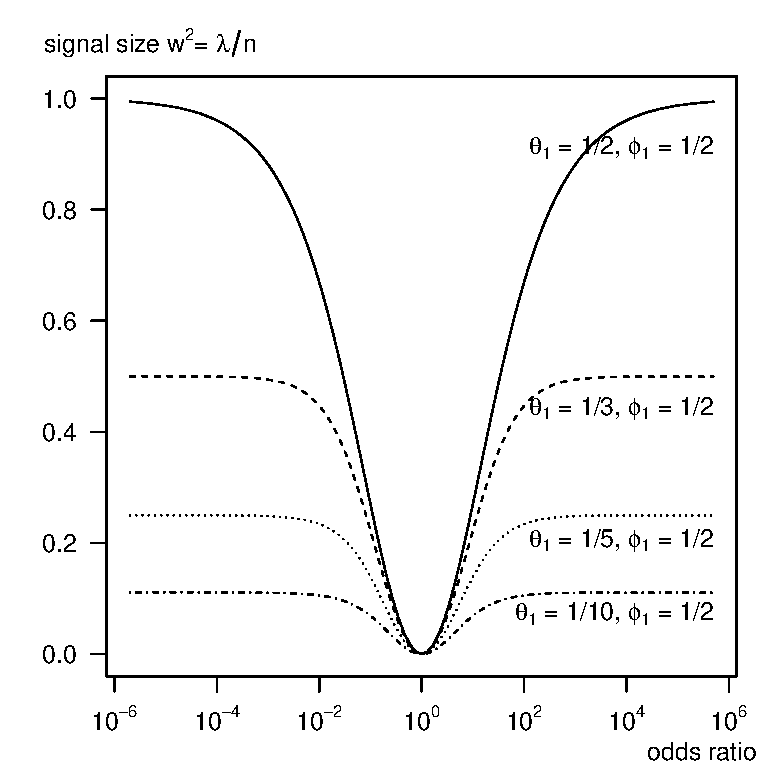
\includegraphics[width=0.49\textwidth]{pics/singal-vs-odds-p05}
      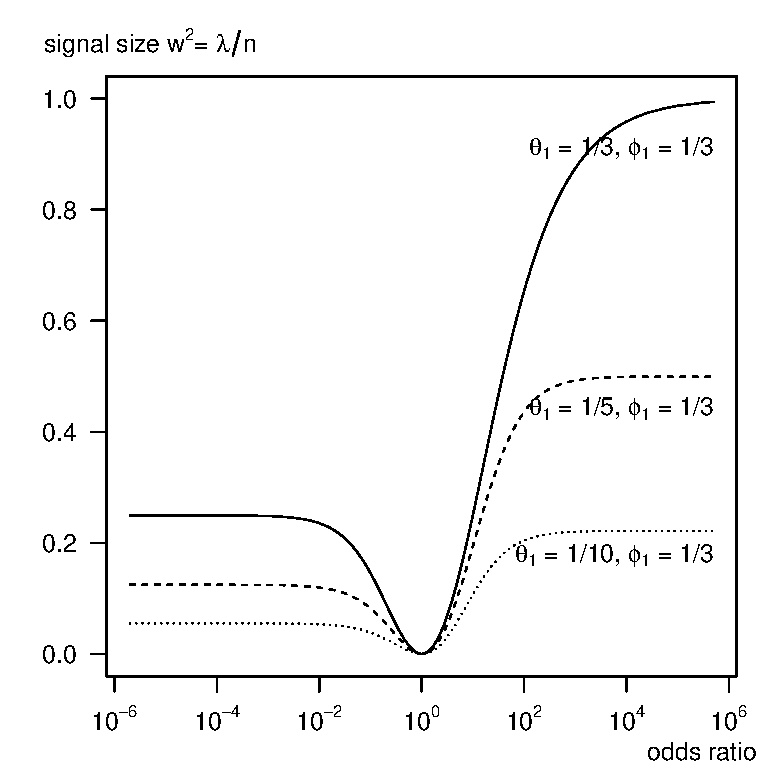
\includegraphics[width=0.49\textwidth]{pics/singal-vs-odds-p0333}            
      \caption{Signal sizes per sample $w^2$ as functions of odds ratios in 2-by-2 multinomial distributions for selected genotype marginals in balanced (left) and unbalanced (right) designs; see Relation \eqref{eq:signal-size-odds-ratio} in Proposition \ref{prop:signal-size-odds-ratio}. For given marginal distributions, extreme odds ratios imply stronger statistical signals at a given sample size. However, the signal sizes are bounded above by constants that depend on the marginal distributions; see Relations \eqref{eq:signal-size-upper-bound-1} and \eqref{eq:signal-size-upper-bound-2}. % Unbalanced marginal distributions -- or rare variants -- lead to smaller signal sizes at a given odds ratio.
      } 
      \label{fig:signal-vs-odds}
\end{figure}

\begin{corollary} \label{cor:signal-limits-OR}
The signal size as a function of the odds ratio $w^2(R)$ is decreasing on $(0,1)$ and increasing on $(1,\infty)$, with limits
\begin{equation} \label{eq:signal-size-upper-bound-1}
    \lim_{\text{R}\to0_+} w^2(\text{R}) = \min\left\{\frac{\phi_1\theta_1}{\phi_2\theta_2}, \frac{\phi_2\theta_2}{\phi_1\theta_1}\right\},
\end{equation}
and
\begin{equation} \label{eq:signal-size-upper-bound-2}
    \lim_{\text{R}\to+\infty} w^2(\text{R}) = \min\left\{\frac{\phi_1\theta_2}{\phi_2\theta_1}, \frac{\phi_2\theta_1}{\phi_1\theta_2}\right\}.
\end{equation}
\end{corollary}
% Proof of Corollary \ref{cor:signal-limits-OR} is found in Appendix \ref{sec:proof-signal-size-odds-ratio}. 

\begin{proof}
	As in the proof of Proposition \ref{prop:signal-size-odds-ratio}, we examine the case where $0<\theta_1,\phi_1\le1/2$, and leave the other three cases an exercise.
	Take the first derivative of the expression for $w^2$ in equation \eqref{eq:signal-size-chisq-delta} with respect to $\delta$, it is evident that $w^2(\delta)$ is decreasing on $[\delta_\mathrm{min},0)$, increasing on $(0,\delta_\mathrm{max}]$, with limits
	$$
	\lim_{d\to \delta_\mathrm{min}} w^2(\delta) = \frac{\phi_1\theta_1}{\phi_2\theta_2},
	\quad
	\text{and}
	\quad
	\lim_{d\to \delta_\mathrm{max}} w^2(\delta) = \min\left\{\frac{\phi_1\theta_2}{\phi_2\theta_1}, \frac{\phi_2\theta_1}{\phi_1\theta_2}\right\}.
	$$
\end{proof}

Corollary \ref{cor:signal-limits-OR} immediately implies that balanced designs with roughly equal number of cases and controls are not necessarily the most informative.

For example, in a study where a third of the recruited subjects carry the genetic variant positively correlated with the trait (i.e., $\theta_1=1/3$), an unbalanced design with $\phi_1=1/3$ would maximize $w^2$ at large odds ratios.
This unbalanced design is much more efficient compared to, say, a balanced design with $\phi_1=1/2$.
In the first case, we have $w^2\to1$ as $R\to\infty$; whereas in the second design, $w^2<1/2$ no matter how large $R$ is.
This difference can also be read by comparing the dashed curve ($\theta_1=1/3$, $\phi_1=1/2$) in the left panel of Figure \ref{fig:signal-vs-odds}, with the solid curve ($\theta_1=1/3$, $\phi_1=1/3$) in the right panel of Figure \ref{fig:signal-vs-odds}.



\section{Optimal study designs and rare variants}
\label{sec:optimal-design} 
For a study with a fixed budget, i.e., a fixed total number of subjects $n$, the researcher is free to choose the fraction of cases $\phi_1$ to be included in the study.
A natural question is how this budget should be allocated to maximize the statistical power of discovery, or equivalently, the signal sizes $\lambda=nw^2$.

In principal, Relation \eqref{eq:signal-size-odds-ratio} can be optimized with respect to the fraction of cases $\phi_1$ in order to find optimal designs, if $\theta_1$ is known and held constant.
In practice, this is not the case.
While the fraction of cases can be controlled, the distributions of genotypes \emph{in the study} are often unknown prior to data collection, and can change with the case-to-control ratio.

Fortunately, the conditional distributions of genotypes in the healthy control groups are often estimated by existing studies, and are made available by consortia such as the NHGRI-EBI GWAS catalog \citep{macarthur2016new}.
% Assume (after appropriate relabelling, hence without loss of generality) that the first variant is associated with an increased risk of disease, and is henceforth referred to as the risk variant.
We denote the conditional frequency of the first genetic variant in the control group as $(f, 1-f)$, where
\begin{equation} \label{eq:RAF}
    f := \mu_{21} / \phi_2.
\end{equation}
The multinomial probability is fully parametrized by the new trio: $(f, \phi_1, R)$.
\begin{center}
    \begin{tabular}{cccc}
    \hline
    & \multicolumn{2}{c}{Genotype} \\
    \cline{2-3}
    Probabilities & Variant 1 & Variant 2 & Total by phenotype \\
    \hline
    Cases & $\frac{\phi_1fR}{fR+1-f}$ & $\frac{\phi_1(1-f)}{fR+1-f}$ & $\phi_1$ \\
    Controls & $f(1-\phi_1)$ & $(1-f)(1-\phi_1)$ & $1-\phi_1$ \\
    \hline
    \end{tabular}
\end{center}
Proposition \ref{prop:signal-size-odds-ratio} may also be re-stated in terms of the new parametrization.

% Note that all these quantities refer to what is in the study, and differ from their counterparts in the general population.

\begin{corollary} \label{cor:signal-size-odds-ratio-conditional-frequency}
In the 2-by-2 multinomial distribution with marginals $(\phi_1, \phi_2 = 1-\phi_1)$, and conditional distribution of the variants in the control group $(f, 1-f)$,
Relation \eqref{eq:signal-size-odds-ratio} holds with $\theta_1 = {\phi_1fR}/{(fR+1-f)} + f(1-\phi_1)$ and $\theta_2 = 1-\theta_1$.
\end{corollary} 

The choice of $\phi_1$ now has a practical solution.

\begin{corollary} \label{cor:optimal-design}
In the context of Corollary \ref{cor:signal-size-odds-ratio-conditional-frequency},
the optimal design $(\phi^*_1, \phi^*_2)$ that maximizes the signal size per sample $w^2$ is prescribed by
\begin{equation} \label{eq:optimal-design}
    \phi_1^* = \frac{fR+1-f}{fR+1-f+\sqrt{R}}, \quad\text{and}\quad 
    \phi_2^* = 1-\phi_1^*.
\end{equation}
% when the denominator in \eqref{eq:optimal-design} is non-zero; otherwise, $\phi_1^*=\phi_2^*=1/2$.
\end{corollary} 


\begin{proof}
	Using the parametrization in \eqref{eq:reparametrize-2-by-2-table-1}, we solve for $\delta$ in \eqref{eq:odds-ratio-delta} to obtain
	\begin{align}
		\delta &= \frac{\phi_1 fR}{fR+1-f} - \left(\frac{\phi_1 fR}{fR+1-f} + f(1-\phi_1)\right)\phi_1 \nonumber \\
		&= \frac{f(1-f)\phi_1(1-\phi_1)(R-1)}{fR+1-f}. \label{eq:reparametrize-2-by-2-table-2}
	\end{align}
	Substituting \eqref{eq:reparametrize-2-by-2-table-2} into the expression \eqref{eq:signal-size-chisq-delta}, after some simplification, yields
	\begin{equation} \label{eq:reparametrize-2-by-2-table-3}
	w^2 = \frac{f(1-f)\phi_1(1-\phi_1)(R-1)^2}{\left[\phi_1 R + (1-\phi_1)D\right]\left[\phi_1 + (1-\phi_1)D\right]},
	\end{equation}
	where $D = fR+1-f > 0$.
	Therefore, he derivative of \eqref{eq:reparametrize-2-by-2-table-3} with respect to $\phi_1$ is
	\begin{equation} \label{eq:signal-size-first-derivative}
	\frac{\mathrm{d}w^2}{\mathrm{d}\phi_1} = 
	\frac{f(1-f)(R-1)^2}{\left[\phi_1 R+(1-\phi_1)D\right]^2 \left[\phi_1+(1-\phi_1)D\right]^2} \left[(D^2-R)\phi_1^2 - 2D^2\phi_1 + D^2\right].
	\end{equation}
	Further, we obtain the second derivative with respect to $\phi_1$,
	\begin{equation} \label{eq:signal-size-second-derivative}
	\frac{\mathrm{d}^2w^2}{\mathrm{d}\phi_1^2} = 
	h(R,f) \left[(\phi_1-1)D^2 - \phi_1R\right],
	\end{equation}
	where $h$ is some function of $(R,f)$ taking on strictly positive values.
	
	Since $\left[(\phi_1-1)D^2 - \phi_1R\right]<0$, the second derivative \eqref{eq:signal-size-second-derivative} must be strictly negative on $[0,1]$.
	This implies that the first derivative \eqref{eq:signal-size-first-derivative} is strictly decreasing on $[0,1]$. 
	Since the first derivative \eqref{eq:signal-size-first-derivative} is strictly positive at $\phi_1=0$, and strictly negative at $\phi_1=1$, it must have a unique zero between 0 and 1, and hence, the solution to $(D^2-R)\phi_1^2 - 2D^2\phi_1 + D^2 = 0$ in the interval of $[0,1]$ must be the maximizer of \eqref{eq:reparametrize-2-by-2-table-3} --- when $D^2-R>0$, the smaller of the two roots maximizes \eqref{eq:reparametrize-2-by-2-table-3}, and when $D^2-R<0$, it is the larger of the two.
	They share the same expression ${D}/{(D+\sqrt{R})}$, which coincides with \eqref{eq:optimal-design}.
	Finally, when $D^2=R$, the only root $\phi_1^*=1/2$, which also coincides with \eqref{eq:optimal-design}, is the maximizer of \eqref{eq:reparametrize-2-by-2-table-3}.
\end{proof}

Of particular interest in the genetics literature are genetic variants with very low allele frequencies in the control group (i.e., $f\approx 0$), known as rare variants.
In such cases, Equation \eqref{eq:optimal-design} can be approximated using the Taylor expansion,
\begin{equation} \label{eq:optimal-design-approx}
    \phi_1^* = \frac{1}{1 + \sqrt{R}} + \frac{(R-\sqrt{R})f}{1+\sqrt{R}} + O(f^2).
\end{equation}
To illustrate, for rare and adversarial factors ($f\approx0$ and $R>1$), the optimal $\phi_1^*$ is less than $1/2$.
Therefore, for studies under a fixed budget, controls should constitute the majority of the subjects, in order to maximize power.
On the other hand, for rare and protective factors ($f\approx0$ and $R<1$), the optimal $\phi_1^*$ is greater than $1/2$, and cases should be the majority.



\section{Phase transitions in large-scale association screening studies}
\label{sec:phase-transitions-in-GWAS}
% Specifically, we develop recipes to find suitable designs of association studies such that combination of the dimensionality $p$, sparsity $\beta$, and signal sizes $r$ of the problem lands in the desired region of risk control, as predicted by the results in Section \ref{sec:chisq-boundaries}.

% Of course, in applications, not all three of the parameters $(p, \beta, r)$ can be altered as we wish.
% In particular, the problem dimensions and sparsity levels are usually determined by the underlying physical processes.
% In the GWAS example, the number of genomic marker locations is determined by the chip used for gene sequencing, while the number of relevant genomic locations is a consequence of the biological process.
% Therefore, in order to achieve a desired level of error control, we can often only hope to influence the statistical signal sizes.

Returning to the problem of \emph{high-dimensional} marginal screenings for categorical covariates, we explore the manifestation of the phase transition in the exact-approximate support recovery problem in the genetic context.

Recall Theorem \ref{thm:chi-squared-exact-approx-boundary} predicts that FWER and FNR can be simultaneously controlled in large dimensions if and only if 
\begin{equation}
    r = \frac{\lambda}{2\log{p}} = \frac{w^2n}{2\log{p}} > 1.
\end{equation}
Therefore, if we were to apply FWER-controlling procedures at low nominal levels (say, $5\%$), then the FNR would experience a phase transition in the sense that, if
\begin{equation} \label{eq:power-1-region}
    r>1 \iff w^2 > \frac{2\log{p}}{n},
\end{equation}
then the FNR can be close to 0; otherwise, FNR must be close to 1.

% Translating this result into the language of association tests, 
Using the parametric relationship described in Corollary \ref{cor:signal-size-odds-ratio-conditional-frequency} (and Proposition \ref{prop:signal-size-odds-ratio}), 
the inequalities in \eqref{eq:power-1-region} implicitly define regions of $(f, R)$ where associations are discoverable with high power, for a given $\phi_1$.
Further, the boundary of such discoverable regions sharpens as dimensionality diverges. 
We illustrate this phase transition through a numerical example next.


\begin{figure}
      \centering
      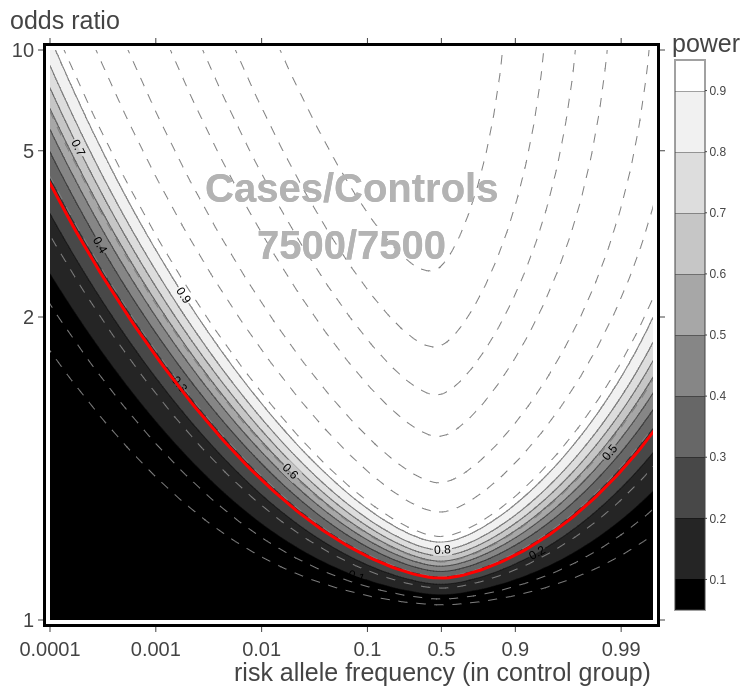
\includegraphics[width=0.49\textwidth]{OR-RAF_plots/OR-RAF_p4.png} 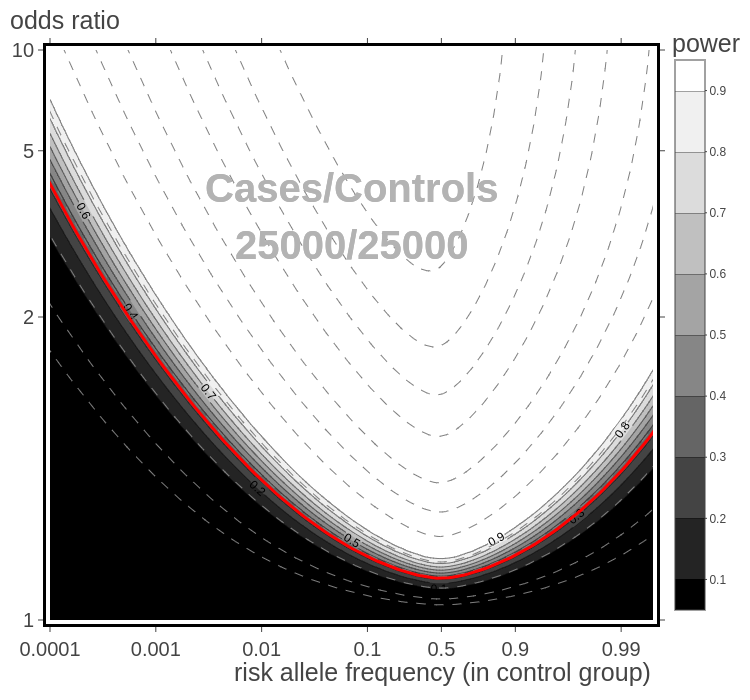
\includegraphics[width=0.49\textwidth]{OR-RAF_plots/OR-RAF_p1e2.png} 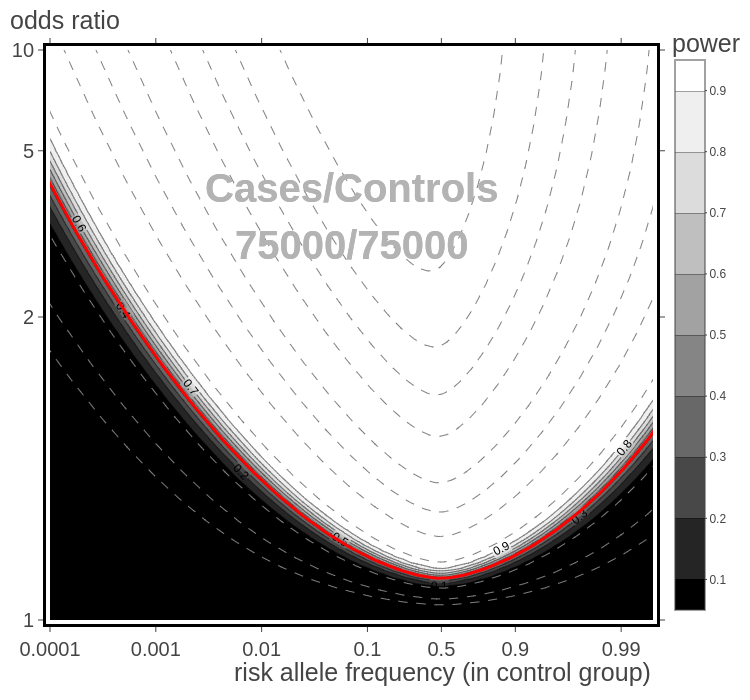
\includegraphics[width=0.49\textwidth]{OR-RAF_plots/OR-RAF_p1e6.png} 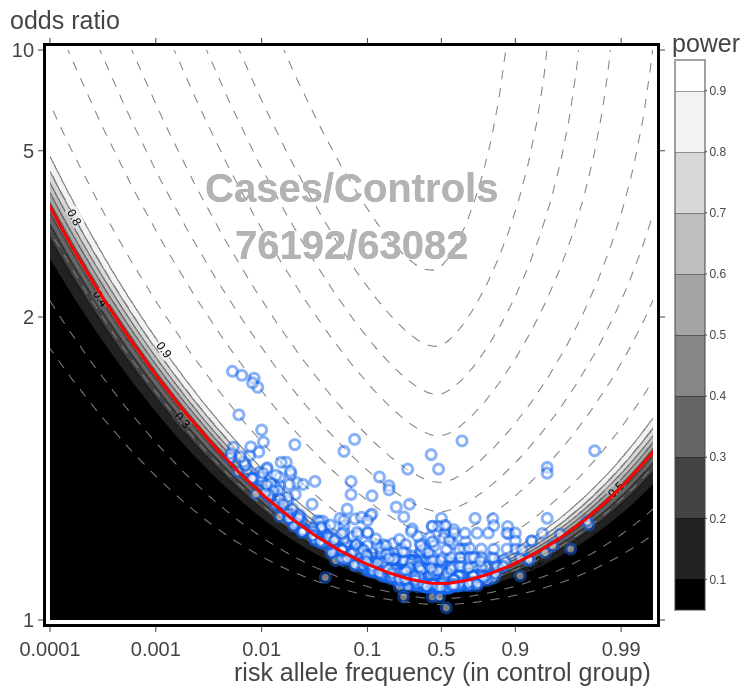
\includegraphics[width=0.49\textwidth]{OR-RAF_plots/OR-RAF_BC_study.png}
      \caption{The OR-RAF diagram visualizing the marginal power of discovery in genetic association studies, after applying Bonferroni's procedure with nominal FWER at $5\%$ level. Sample sizes are marked in each panel, and the problem dimensions are, respectively, $p=4$ (upper-left), $p=10^2$ (upper-right), and $p=10^6$ (lower-left), so that $n/\log{p}$ are roughly constant. Red curves mark the boundaries ($r=1$) of the phase transition for the exact-approximate support recovery problem; dashed curves are the equi-signal (equi-power) curves. The phase transition in signal sizes $\lambda$ translates into the phase transition in terms of $(f,R)$, and sharpens as $p\to\infty$; see Example \ref{exmp:OR-RAF_phase_transition}. In the lower-right panel, we visualize discovered associations (blue circles) in a recent GWA study (Michailidou et al. (2017)); the estimated odds ratios and risk allele frequencies are subject to survival bias and should not be taken at their face values; see Remark \ref{rmk:OR-RAF_false_evidence}.
      } 
      \label{fig:OR-RAF_GWAS}
\end{figure}


\begin{example}
\label{exmp:OR-RAF_phase_transition}
Consider association tests on $2\times2$ contingency tables at $p$ locations as introduced in Section \ref{sec:motivation-chisq}, where the counts follow 
a multinomial distribution
% independent binomial distributions 
% $$
% O_{11} \sim \mathrm{Binom}(n\phi_1, fR/(fR+1-f)),\quad 
% O_{21} \sim \mathrm{Binom}(n(1-\phi_1), fR/(fR+1-f)),
% $$
parametrized by $(f, R, \phi_1)$ as in Section \ref{sec:optimal-design}.
Assume that the phenotype marginals are fixed at $\phi_1 = \phi_2 = 1/2$.
% --- as is the case in genetic association studies --- 
Applying Bonferroni's procedure with nominal FWER at $\alpha=5\%$ level, we can approximate the marginal power of association tests by
\begin{equation} \label{eq:power-approximation}
    \P[\chi^2_{1}(\lambda)>\chi^2_{1,\alpha/p}],
\end{equation}
where $\chi^2_{1,\alpha/p}$ is the upper $(\alpha/p)$-quantile of a central chi-squared distribution with 1 degree of freedom.
We calculate this marginal power as a function of the parameters $(f,R)$ in three scenarios:
\begin{itemize}
    \item $p=4$, $n=3\times10^4$ 
    \item $p=10^2$, $n=1\times10^5$
    \item $p=10^6$, $n=3\times10^6$
\end{itemize}
and visualize the results as heatmaps\footnote{Since genetic variants can always be relabelled such that Variant 1 is positively associated with Cases, we only produce part of the diagram where $R>1$.
Sample sizes marked in the figure are adjusted by a factor of $1/2$, to reflect the genetic context where a pair of alleles are measured for every individual at every genomic location.} (referred to as OR-RAF diagrams) in Figure \ref{fig:OR-RAF_GWAS}.
These parameter values are chosen so that $\log{p}/n$ are roughly constant (around $4.6\times10^{-5}$).

We also overlay ``equi-signal'' curves, i.e., functions implicitly defined by the equations $r=c$ for a range of $c$ (dashed curves), and highlight the predicted boundary of phase transition for the exact-approximate support recovery problem $r=1$ (red curves).
The change in marginal power clearly sharpens around the predicted boundary $r=1$ as dimensionality diverges.
\end{example}

% --- or equivalently, the marginal power ---


\begin{remark}
\label{rmk:OR-RAF_false_evidence}
In an attempt to find empirical evidence of our theoretical predictions, we chart the genetic variants associated with breast cancer, discovered in a 2017 study by \citet{michailidou2017association} in an OR-RAF diagram. 
The estimated risk allele frequencies ($f$) and odds ratios ($R$) are taken from the NHGRI-EBI GWAS catalog \cite{macarthur2016new}, and plotted against a power heatmap calculated according to the reported sample sizes. 
See lower-right panel of Figure \ref{fig:OR-RAF_GWAS}.

It is tempting to believe, on careless inspection, that roughly \emph{all} discovered associations fall inside the high power region of the diagram, therefore demonstrating the phase transition in statistical power.
Unfortunately, the estimates here are subject to survival {bias} --- the study in fact uses the {same} dataset for \emph{both} support estimation and parameter estimation, without adjusting the latter for the selection process.
The seemingly striking agreement between the power calculations and the estimated effects of reported associations \emph{should not} be taken as evidence for the validity of our theory.
We conjecture, as the theory predicts, that accurate and unbiased parameter estimates from an independent replication will still place the associations in the high power region of the diagram. 
\end{remark}

Finally, we demonstrate with an example how results in Sections \ref{sec:chisq-boundaries} and \ref{sec:odds-and-power} may be used for planning prospective association studies.

\begin{example}
In a GWAS with $p = 10^6$ genomic marker locations, researchers wish to locate genetic associations with the trait of interest.
Specifically, they wish to maximize power in the region where genetic variants have risk allele frequencies of $0.01$ and odds ratios of $1.2$.
By Corollary \ref{cor:optimal-design}, the optimal design has a fraction of cases $\phi^* = 0.478$, yielding the statistical signal size per sample $w^2\approx9.00\times10^{-5}$ according to Corollary \ref{cor:signal-size-odds-ratio-conditional-frequency}.

If we wish to achieve exact-approximate support recovery in the sense of \eqref{eq:support-recovery-success}, Theorem \ref{thm:chi-squared-exact-approx-boundary} predicts that the signal size parameter $r$ has to be at least $\widetilde{g}(\beta)= 1$.
This signal size calls for a sample size of $n = \lambda / w^2 = 2r\log(p)/w^2 \approx 307,011$.
In a typically GWAS, a pair of alleles are sequenced for every marker location, bringing the required number of subjects in the study to $n/2 \approx 153,509$.
\end{example}

In comparison, a more accurate power calculation directly using \eqref{eq:power-approximation} predicts that $n / 2 = 165,035$ subjects are needed, under the set of parameters ($p=10^6$, $f=0.01$, $R=1.2$) and $\mathrm{FWER}=0.05$, $\mathrm{FNR}=0.5$; this is $7\%$ higher than our crude asymptotic approximation.
% The accuracy of the asymptotic approximations, by nature of the statements in Theorem \ref{thm:chi-squared-exact-boundary} and \ref{thm:chi-squared-approx-boundary}, depends on how close the error metrics are to zero.
% For example, the number of subjects needed for $\mathrm{FWER}=\mathrm{FWNR}=0.01$ is $499,598$, an $8\%$ increase over the asymptotic prediction; at $\mathrm{FWER}=\mathrm{FWNR}=0.1$, this number becomes $398,996$, some $14\%$ lower than the asymptotic result.
In general, we recommend using the more precise calculations over the back-of-the-envelope asymptotics for planning prospective studies and performing systematic reviews;
a user-friendly web application implementing the more precise approximations is provided in \cite{gao2019upass}.
Nevertheless, the theoretical results on phase transitions generate simple, accurate, and powerful insights that cannot be easily derived from numerical calculations.




\section{Numerical illustrations of the phase transitions in chi-square models}
\label{sec:numerical}
We illustrate with simulations the phase transition phenomena in the chi-square model, and compare numerically the required signal sizes in support recovery problems between the two types of alternatives in the additive error model.
% We also demonstrate the fundamental trade-off between odds ratios and relative frequencies in association studies, as outlined in Proposition \ref{prop:signal-size-odds-ratio} and Corollary \ref{cor:signal-size-odds-ratio-conditional-frequency}, using evidence from large-scale genetic studies.

\subsection{Exact support recovery}

The sparsity of the signal vectors in the experiments are parametrized as in \eqref{eq:signal-sparsity}. 
Signal sizes are assumed equal with magnitude $\lambda(i)=2r\log{p}$ for $i\in S$.
We estimate the support set $S$ using Bonferroni's procedure with nominal FWER level set at $1/(5{\log{p}})$.
The nominal FWER levels vanishes slowly, in line with the assumptions in Theorem \ref{thm:chi-squared-exact-boundary}.
Experiments were repeated 1000 times at each of the 400 sparsity-signal-size combinations, for dimensions $p=10^2, 10^3$, and $10^4$.

The empirical probabilities of exact support recovery under Bonferroni's procedure are shown in Figure \ref{fig:phase-simulated-chi-squared}.
The numerical results suggest not only good accuracy of the predicted boundaries in high-dimensions ($p=10^4$, right panels of Figure \ref{fig:phase-simulated-chi-squared}), but also practical relevance of the theoretical predictions in moderate dimensions ($p=100$, left panels of Figure \ref{fig:phase-simulated-chi-squared}).

\begin{figure}
      \centering
      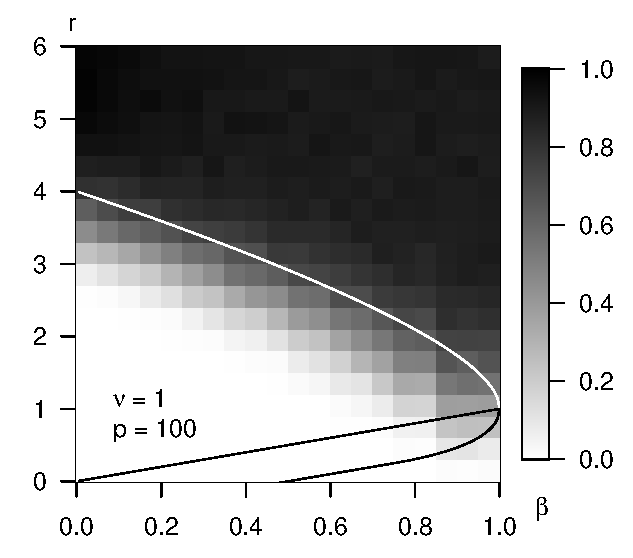
\includegraphics[width=0.32\textwidth]{sim_strong_boundary/simulated_phase_diagram_chi-squared_nu1_p100.eps}
      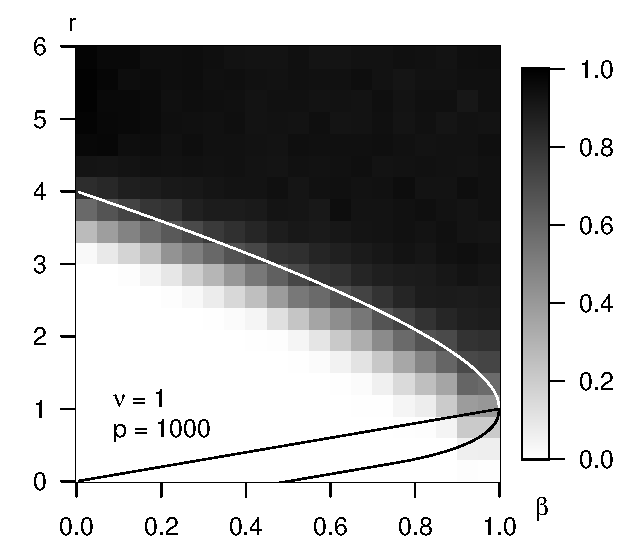
\includegraphics[width=0.32\textwidth]{sim_strong_boundary/simulated_phase_diagram_chi-squared_nu1_p1000.eps}
      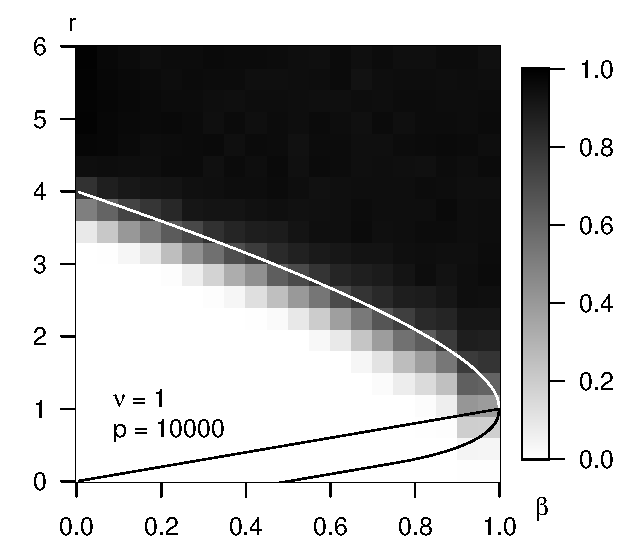
\includegraphics[width=0.32\textwidth]{sim_strong_boundary/simulated_phase_diagram_chi-squared_nu1_p10000.eps}
      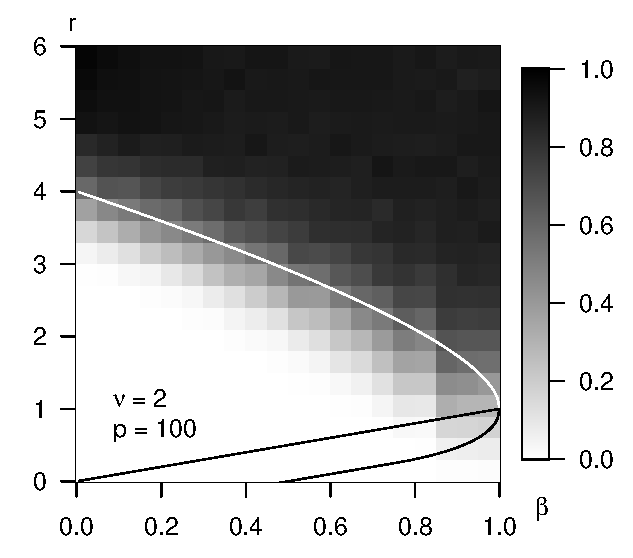
\includegraphics[width=0.32\textwidth]{sim_strong_boundary/simulated_phase_diagram_chi-squared_nu2_p100.eps}
      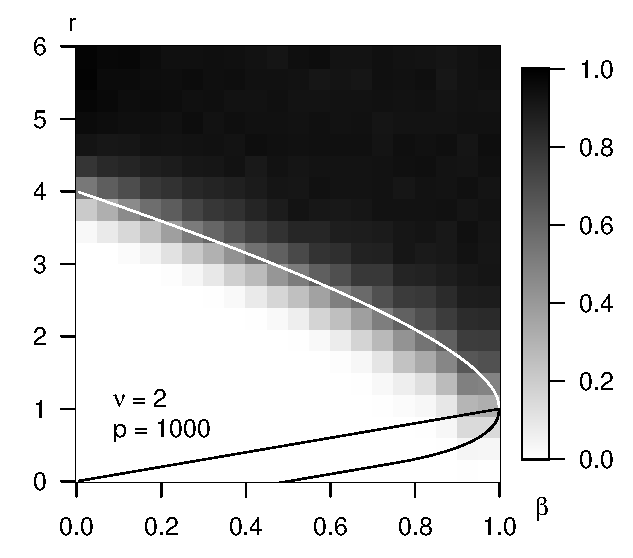
\includegraphics[width=0.32\textwidth]{sim_strong_boundary/simulated_phase_diagram_chi-squared_nu2_p1000.eps}
      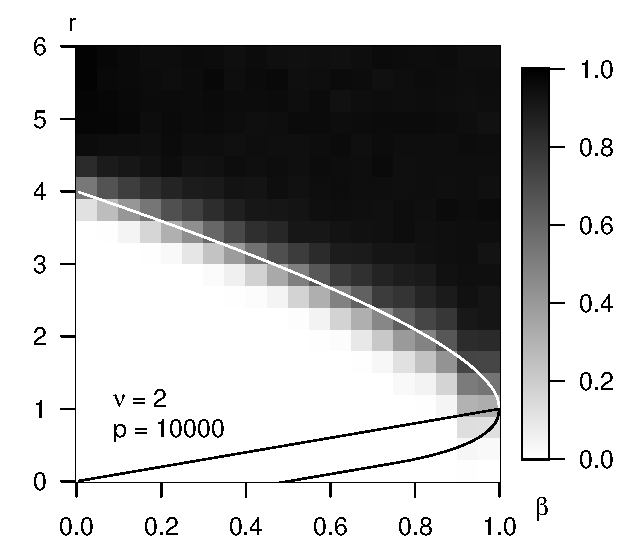
\includegraphics[width=0.32\textwidth]{sim_strong_boundary/simulated_phase_diagram_chi-squared_nu2_p10000.eps}
      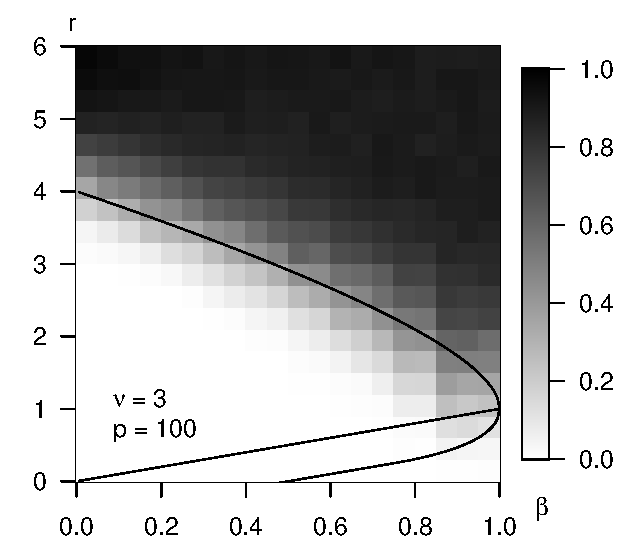
\includegraphics[width=0.32\textwidth]{sim_strong_boundary/simulated_phase_diagram_chi-squared_nu3_p100.eps}
      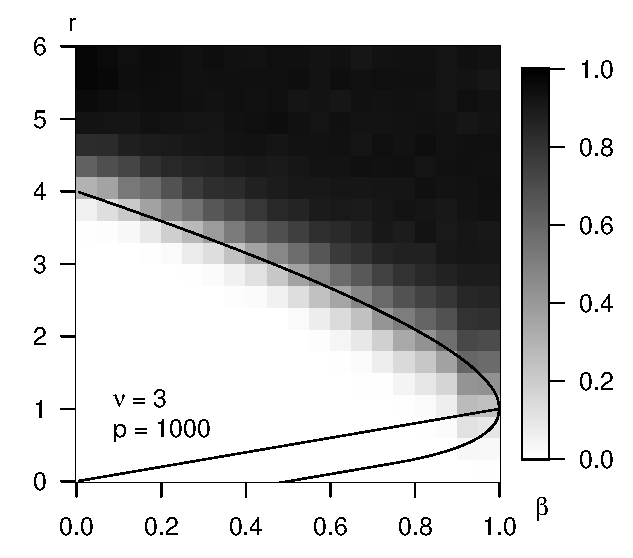
\includegraphics[width=0.32\textwidth]{sim_strong_boundary/simulated_phase_diagram_chi-squared_nu3_p1000.eps}
      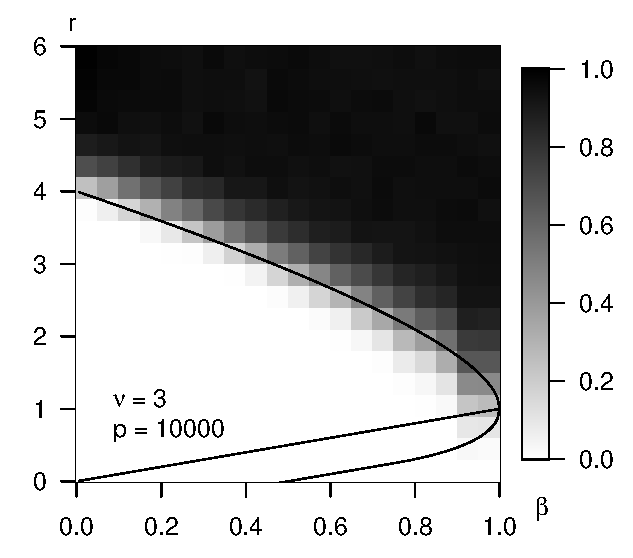
\includegraphics[width=0.32\textwidth]{sim_strong_boundary/simulated_phase_diagram_chi-squared_nu3_p10000.eps}
      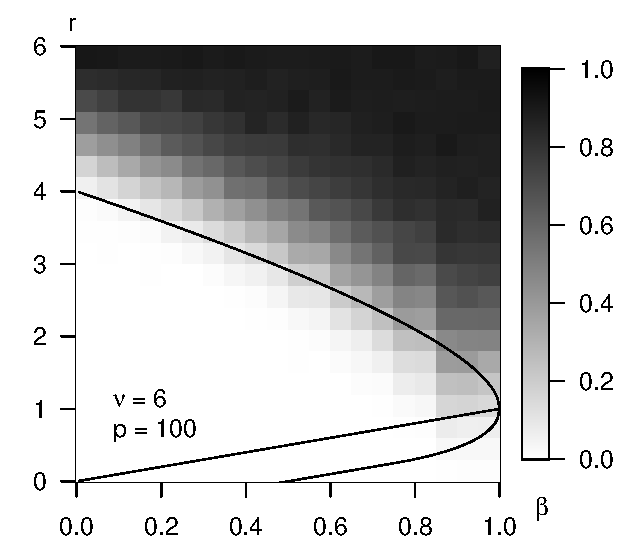
\includegraphics[width=0.32\textwidth]{sim_strong_boundary/simulated_phase_diagram_chi-squared_nu6_p100.eps}
      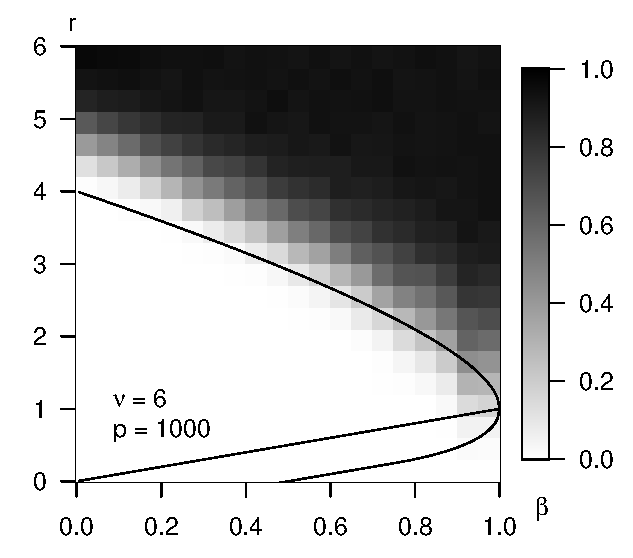
\includegraphics[width=0.32\textwidth]{sim_strong_boundary/simulated_phase_diagram_chi-squared_nu6_p1000.eps}
      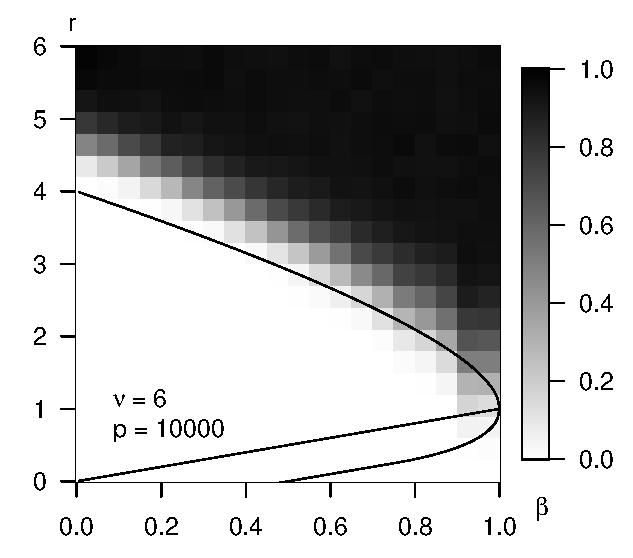
\includegraphics[width=0.32\textwidth]{sim_strong_boundary/simulated_phase_diagram_chi-squared_nu6_p10000.eps}
      \caption{The empirical probability of exact support recovery of Bonferroni's procedure in the chi-squared model \eqref{eq:model-chisq}. 
      We simulate $\nu=1, 2, 3, 6$ (first to last row), at dimensions $p=10^2, 10^3, 10^4$ (left to right column), for a grid of sparsity levels $\beta$ and signal sizes $r$.
      The experiments were repeated 1000 times for each sparsity-signal size combination; darker color indicates higher probability of exact support recovery.  
      Numerical results are in general agreement with the boundaries described in Theorem \ref{thm:chi-squared-exact-boundary}; for large $\nu$'s, the phase transitions take place somewhat above the predicted boundaries.
      The boundary for the approximate support recovery (Theorem \ref{thm:chi-squared-approx-boundary}) and the detection boundary (see Donoho and Jin (2004)) are plotted for comparison.} 
      \label{fig:phase-simulated-chi-squared}
\end{figure}

We conduct further experiments to examine the optimality claims in Theorem \ref{thm:chi-squared-exact-boundary} by comparing with the oracle procedure with thresholds $t_p=\min_{i\in S}x(i)$.
We also examine the claims in Section \ref{subsec:one-vs-two-sided}, and compare the one-sided alternatives in Gaussian additive models with the two-sided alternatives (or equivalently, the chi-square model with $\nu=1$).
We apply Bonferroni's procedure and the oracle thresholding procedure in both settings.

Experiments were repeated 1000 times for a grid of signal size values ranging from $r=0$ to $6$, and for dimensions $10^2, 10^3$, and $10^5$.
Results of the experiments, shown in Figure \ref{fig:one-vs-two-sided-exact_support_recovery}, suggest vanishing difference between difficulties of two-sided vs one-sided alternatives in the additive error models, as well as vanishing difference between the powers of Bonferroni's procedures and the oracle procedures as $p\to\infty$.

\begin{figure}
      \centering
      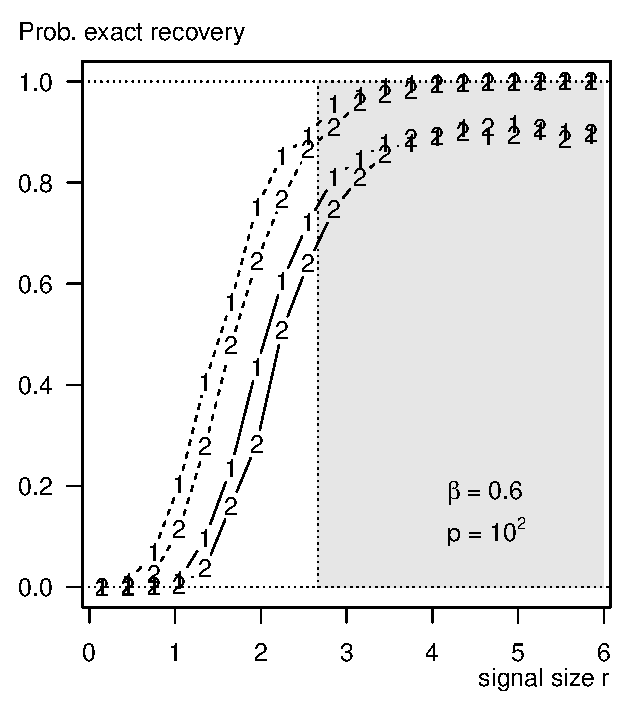
\includegraphics[width=0.32\textwidth]{sim_one-vs-two-sided/exact_recovery_one-vs-two-sided_beta06_p100.eps}
      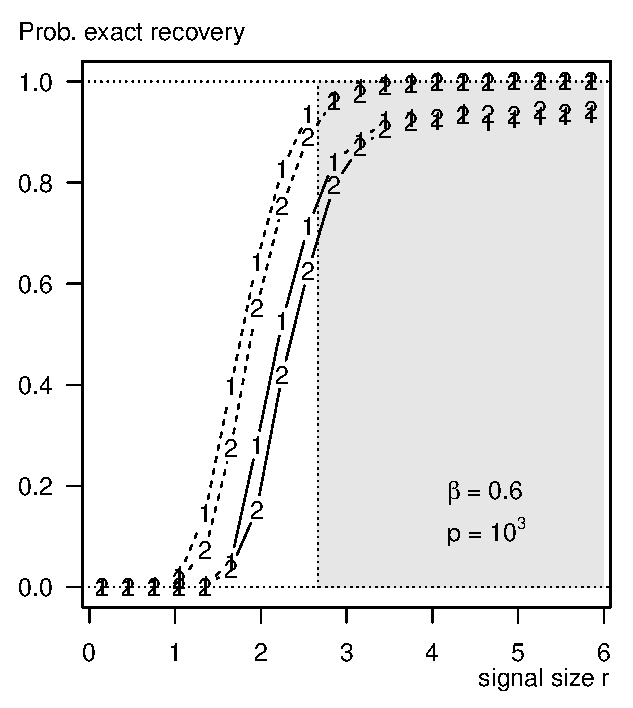
\includegraphics[width=0.32\textwidth]{sim_one-vs-two-sided/exact_recovery_one-vs-two-sided_beta06_p1000.eps}
      % 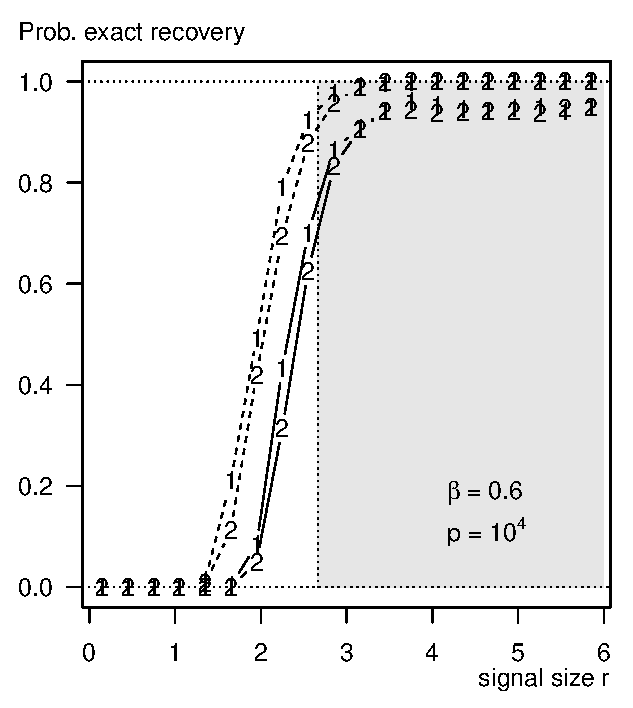
\includegraphics[width=0.33\textwidth]{sim_one-vs-two-sided/exact_recovery_one-vs-two-sided_beta06_p10000.eps}
      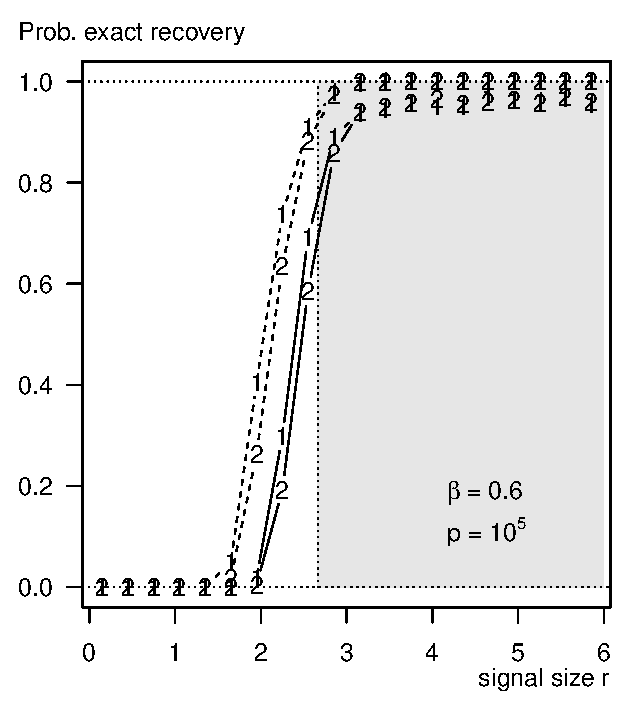
\includegraphics[width=0.32\textwidth]{sim_one-vs-two-sided/exact_recovery_one-vs-two-sided_beta06_p100000.eps}
      \caption{The empirical probability of exact support recovery of Bonferroni's procedure (solid curves) and the oracle procedure (dashed curves) in the chi-squared model with one degree of freedom (marked `2') in the additive Gaussian error model and under one-sided alternatives (marked `1'). 
      We simulate at dimensions $p=10^2, 10^3, 10^5$ (left to right) for a grid of signal sizes $r$ and sparsity level $\beta=0.6$.
      The experiments were repeated 1000 times for each method-model-signal-size combination. 
      Numerical results show evidence of convergence to the 0-1 law as predicted by Theorem \ref{thm:chi-squared-exact-boundary}; regions where asymptotically exact support recovery can be achieved are shaded in grey.
      The difference in power between Bonferroni's procedure and the oracle procedure, as well as in the two types of alternatives both decrease as dimensionality increases.} 
      \label{fig:one-vs-two-sided-exact_support_recovery}
\end{figure}

\subsection{Approximate, and approximate-exact support recovery}

Similar experiments are conducted to examine the optimality claims in Theorem \ref{thm:chi-squared-approx-boundary}, and in Section \ref{subsec:one-vs-two-sided}.
We define an oracle thresholding procedure for approximate support recovery, where the threshold is chosen to minimize the empirical risk.
That is,
$$
t_p(x, S) \in \argmin_{t\in\R} \frac{|\widehat{S}(t)\setminus S|}{\max\{|\widehat{S}(t)|,1\}} + \frac{|S\setminus \widehat{S}(t)|}{\max\{|{S}|,1\}},
%\mathcal{R^\mathrm{oracle}} \in \argmin_{\widehat{S}(\mathcal{R})\in\mathcal{S}} \mathrm{risk}^{\mathrm{A}}(\mathcal{R}),
$$
where $\widehat{S}(t) = \{i\;|\;x(i)\ge t\}$;
in implementation, we only need to scan the values of observations $t\in\{x(1), \ldots, x(p)\}$. 
The nominal FDR level for the BH procedure is set at $1/(5{\log{p}})$, therefore slowly vanishing, in line with the assumptions in Theorem \ref{thm:chi-squared-approx-boundary}; all other parameters are identical to that in the experiments for exact support recovery.
Results of the experiments are shown in Figure \ref{fig:one-vs-two-sided-approx_support_recovery} and Figure \ref{fig:phase-simulated-chi-squared-approx-boundary}.

We also examine the boundary described in Theorem \ref{thm:chi-squared-exact-approx-boundary}.
Experimental settings are identical to that in the experiments for approximate support recovery.
% Results for the BH procedure are in general close to that of the oracle procedure,
We compare the performance of the BH procedure with an oracle procedure with threshold
$$
t_p(x, S) \in \min_{i\in S} x(i),
$$
and visualize results of the experiments in Figure \ref{fig:phase-simulated-chi-squared-approx-exact-boundary}.
Notice that the BH procedure sets its threshold somewhat higher than the oracle, especially for small $\beta$'s. 
The empirical risk of the oracle procedure (not shown here in the interest of space) follows much more closely the predicted boundary \eqref{eq:approx-exact-boundary-chisquared}.

\begin{figure}
      \centering
      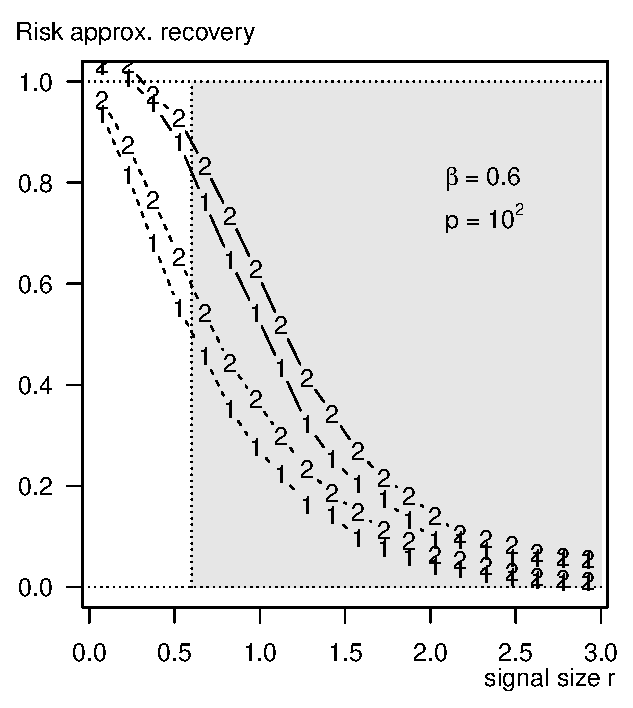
\includegraphics[width=0.32\textwidth]{sim_one-vs-two-sided/approx_recovery_one-vs-two-sided_beta06_p100.eps}
      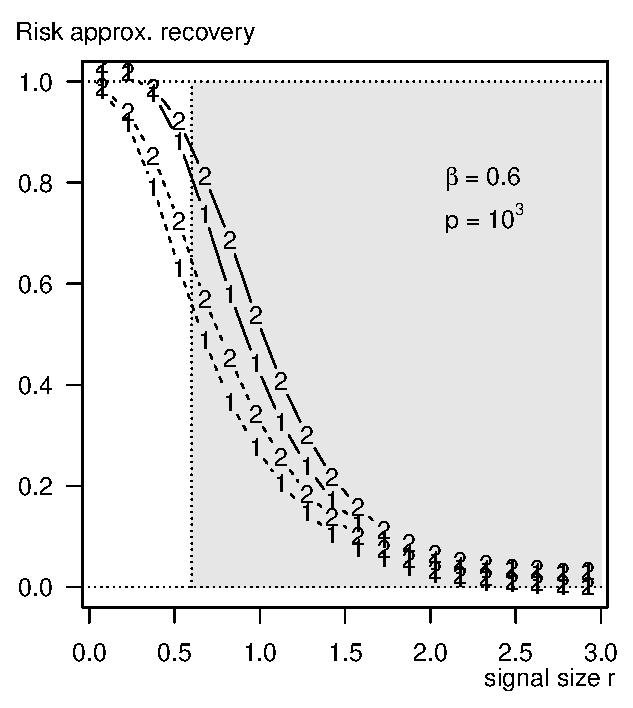
\includegraphics[width=0.32\textwidth]{sim_one-vs-two-sided/approx_recovery_one-vs-two-sided_beta06_p1000.eps}
      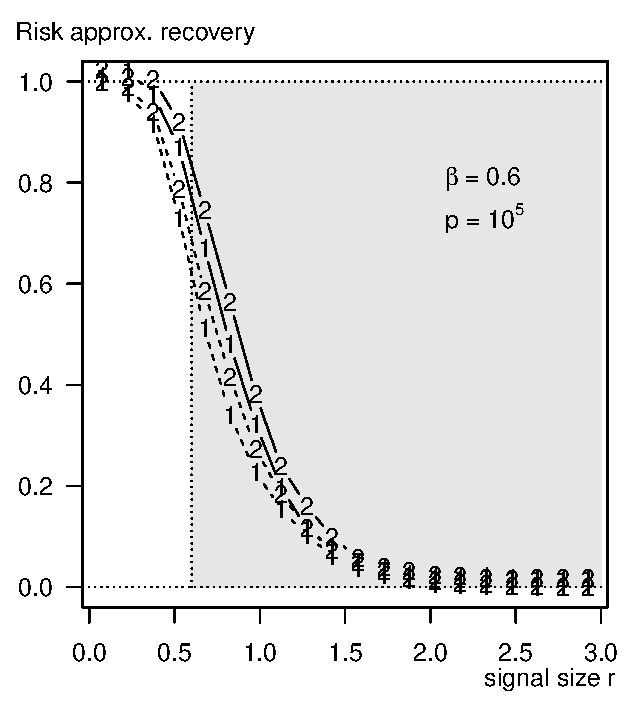
\includegraphics[width=0.32\textwidth]{sim_one-vs-two-sided/approx_recovery_one-vs-two-sided_beta06_p100000.eps}
      \caption{The empirical risk of approximate support recovery of Benjamini-Hochberg's procedure (solid curves) and the oracle procedure (dashed curves) in the chi-squared model with one degree of freedom (marked `2') and in the additive Gaussian error model under one-sided alternatives (marked `1'). 
      We simulate at dimensions $p=10^2, 10^3, 10^5$ (left to right) for a grid of signal sizes $r$ and sparsity level $\beta=0.6$.
      The experiments were repeated 1000 times for each method-model-signal-size combination. 
      Numerical results show evidence of convergence to the 0-1 law as predicted by Theorem \ref{thm:chi-squared-approx-boundary}; regions where asymptotically approximate support recovery can be achieved are shaded in grey.
      The difference in risks between Benjamini-Hochberg's procedure and the oracle procedure, as well as in the two types of alternatives, both decrease as dimensionality increases.} 
      \label{fig:one-vs-two-sided-approx_support_recovery}
\end{figure}


\begin{figure}
      \centering
      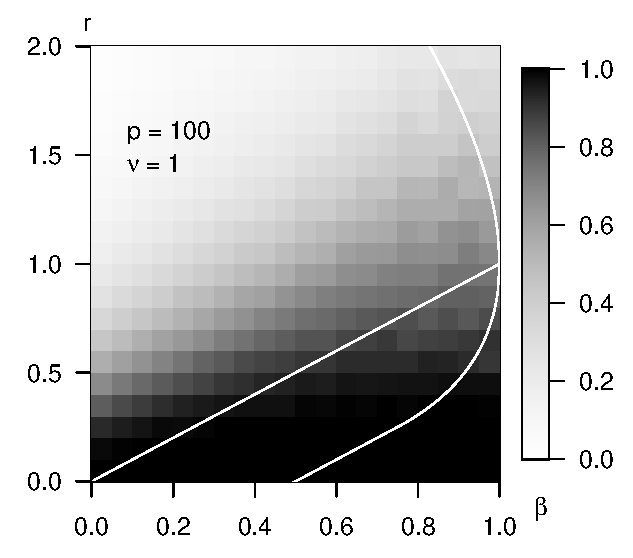
\includegraphics[width=0.32\textwidth]{sim_weak_boundary/simulated_weak_boundary_chi-squared_nu1_p100.eps}
      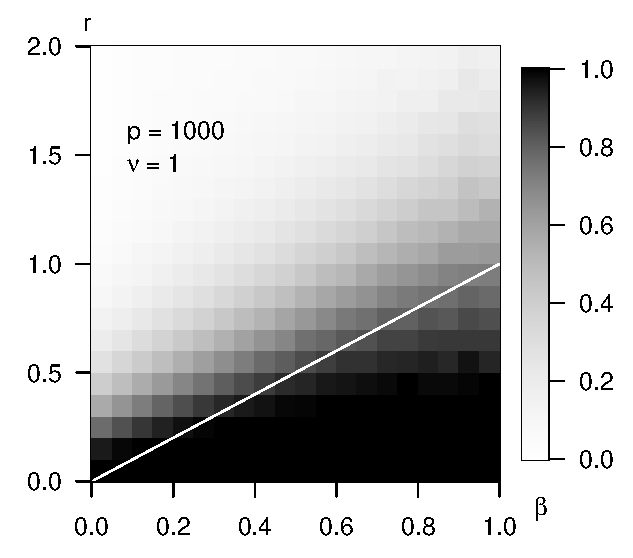
\includegraphics[width=0.32\textwidth]{sim_weak_boundary/simulated_weak_boundary_chi-squared_nu1_p1000.eps}
      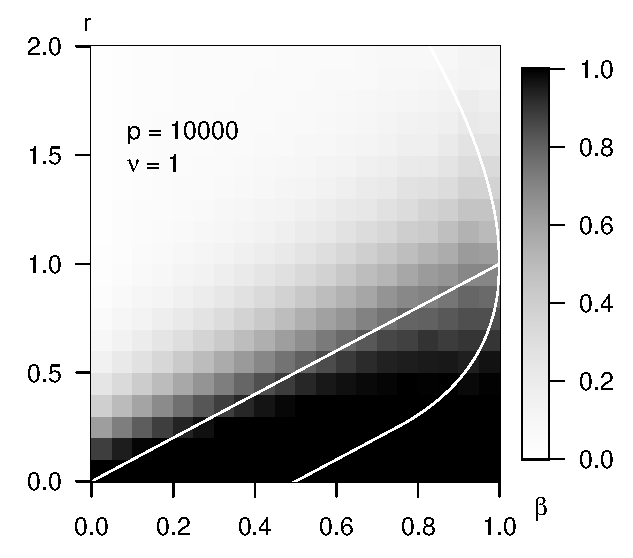
\includegraphics[width=0.32\textwidth]{sim_weak_boundary/simulated_weak_boundary_chi-squared_nu1_p10000.eps}
      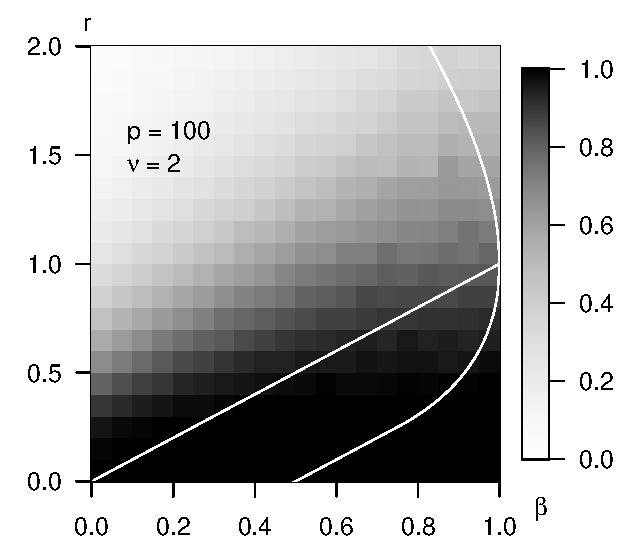
\includegraphics[width=0.32\textwidth]{sim_weak_boundary/simulated_weak_boundary_chi-squared_nu2_p100.eps}
      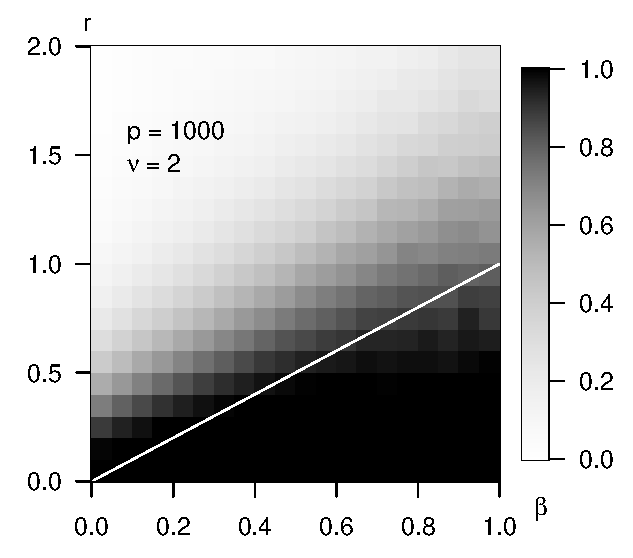
\includegraphics[width=0.32\textwidth]{sim_weak_boundary/simulated_weak_boundary_chi-squared_nu2_p1000.eps}
      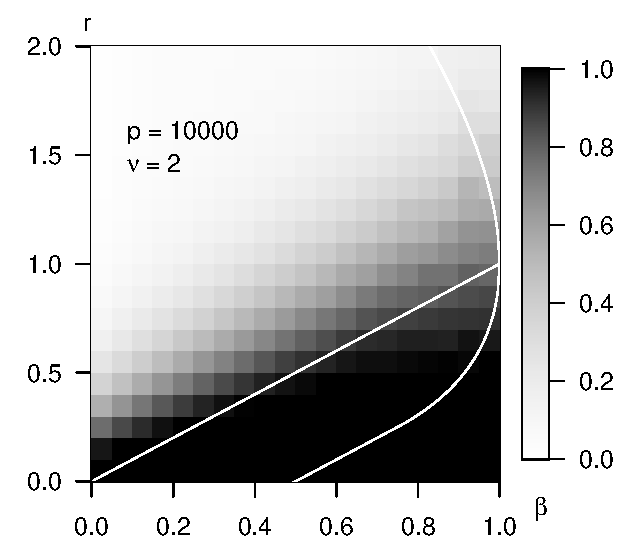
\includegraphics[width=0.32\textwidth]{sim_weak_boundary/simulated_weak_boundary_chi-squared_nu2_p10000.eps}
      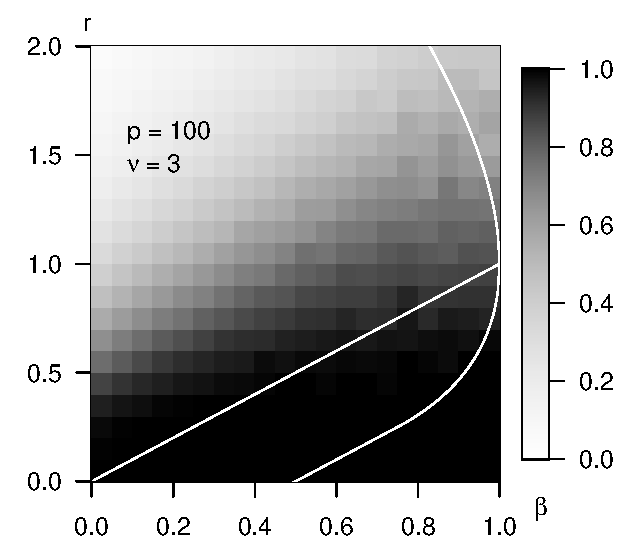
\includegraphics[width=0.32\textwidth]{sim_weak_boundary/simulated_weak_boundary_chi-squared_nu3_p100.eps}
      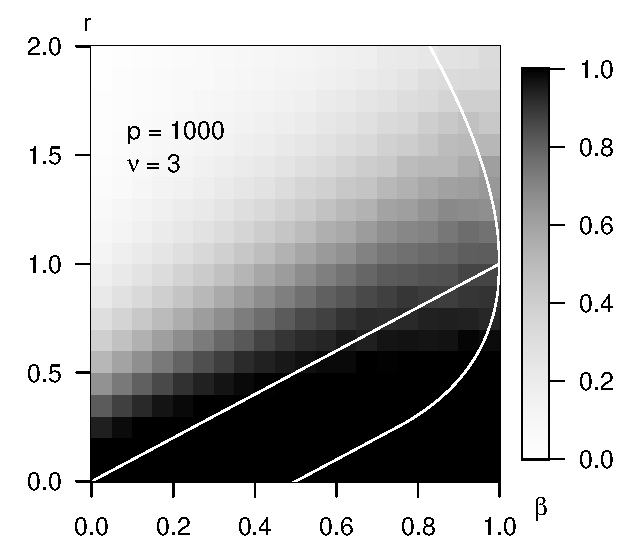
\includegraphics[width=0.32\textwidth]{sim_weak_boundary/simulated_weak_boundary_chi-squared_nu3_p1000.eps}
      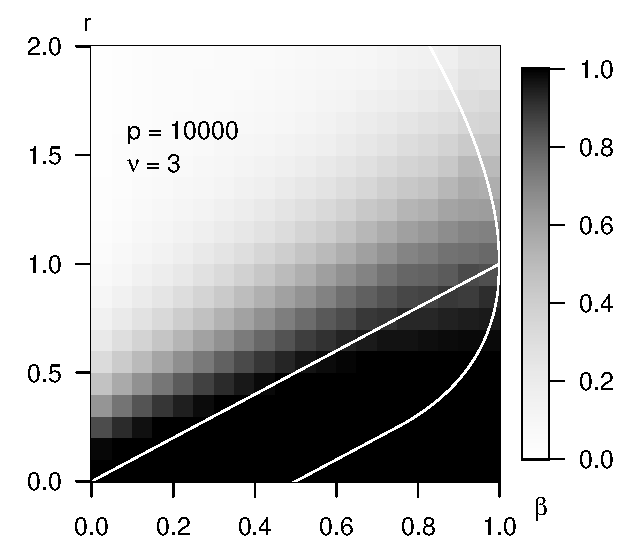
\includegraphics[width=0.32\textwidth]{sim_weak_boundary/simulated_weak_boundary_chi-squared_nu3_p10000.eps}
      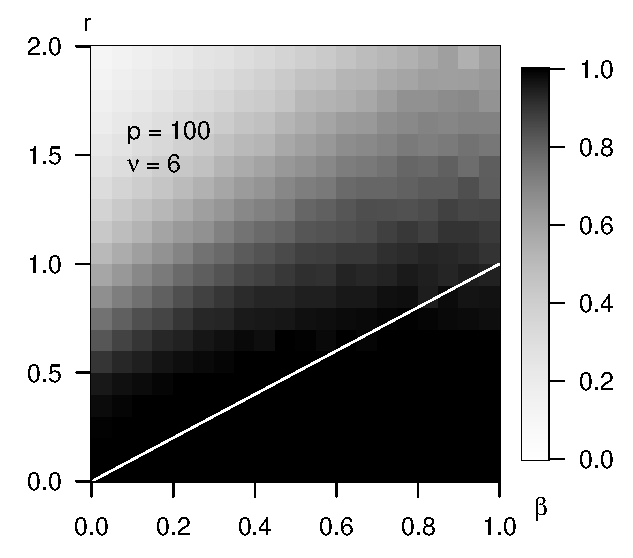
\includegraphics[width=0.32\textwidth]{sim_weak_boundary/simulated_weak_boundary_chi-squared_nu6_p100.eps}
      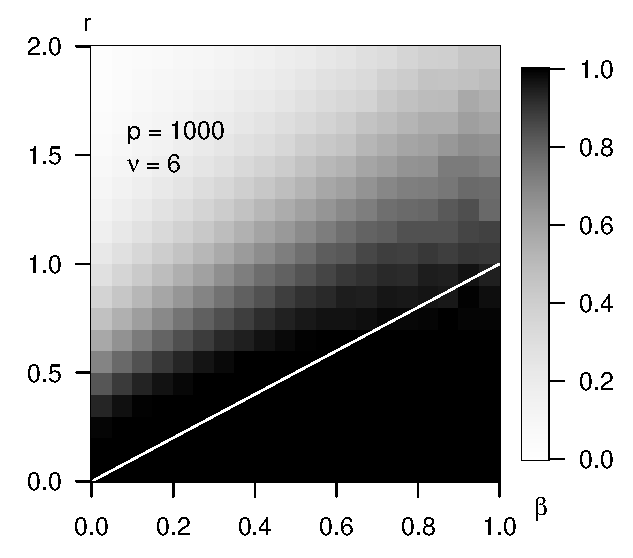
\includegraphics[width=0.32\textwidth]{sim_weak_boundary/simulated_weak_boundary_chi-squared_nu6_p1000.eps}
      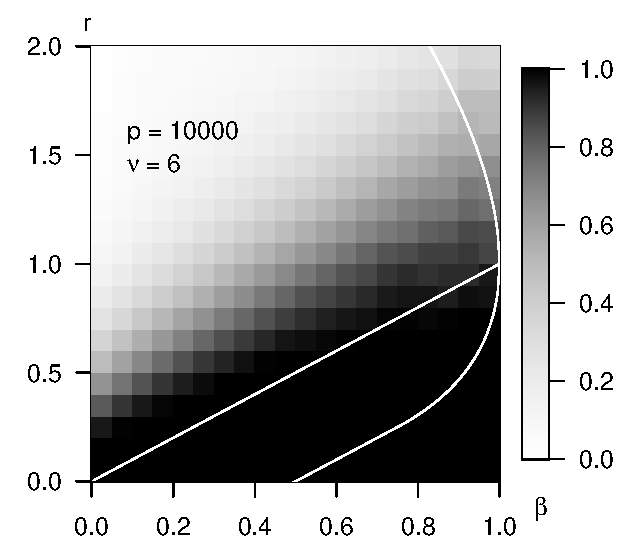
\includegraphics[width=0.32\textwidth]{sim_weak_boundary/simulated_weak_boundary_chi-squared_nu6_p10000.eps}
      \caption{The estimated risk of approximate support recovery $\mathrm{risk}^{\mathrm{A}}$ (see \eqref{eq:risk-approximate}) of the Benjamini-Hochberg procedure in the chi-squared model \eqref{eq:model-chisq}. 
      We simulate $\nu=1, 2, 3, 6$ (first to last row), at dimensions $p=10^2, 10^3, 10^4$ (left to right column), for a grid of sparsity levels $\beta$ and signal sizes $r$.
      The experiments were repeated 1000 times for each sparsity-signal size combination; darker color indicates higher larger $\mathrm{risk}^{\mathrm{A}}$. 
      Numerical results are generally in agreement with the boundaries described in Theorem \ref{thm:chi-squared-approx-boundary}; for large $\nu$'s, the phase transitions take place somewhat above the predicted boundaries.
      The boundary for the exact support recovery problem (Theorem \ref{thm:chi-squared-exact-boundary}) and the detection boundary (see Donoho and Jin (2004)) are plotted for comparison.} 
      \label{fig:phase-simulated-chi-squared-approx-boundary}
\end{figure}


\begin{figure}
      \centering
      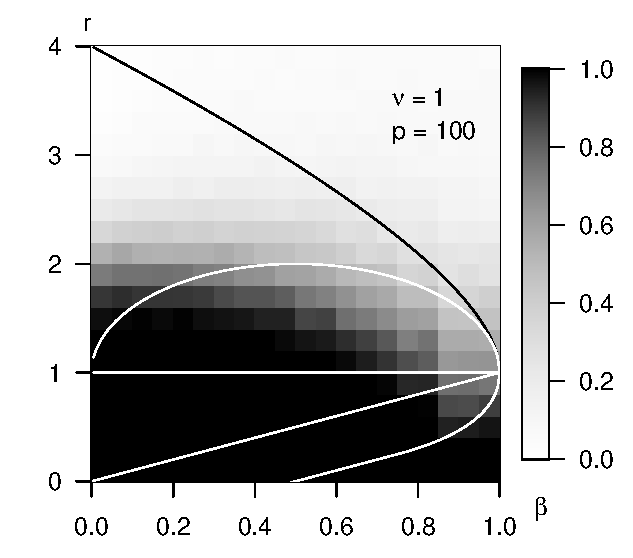
\includegraphics[width=0.32\textwidth]{sim_approx-exact_boundary/simulated_approx-exact_boundary_chi-squared_nu1_p100.eps}
      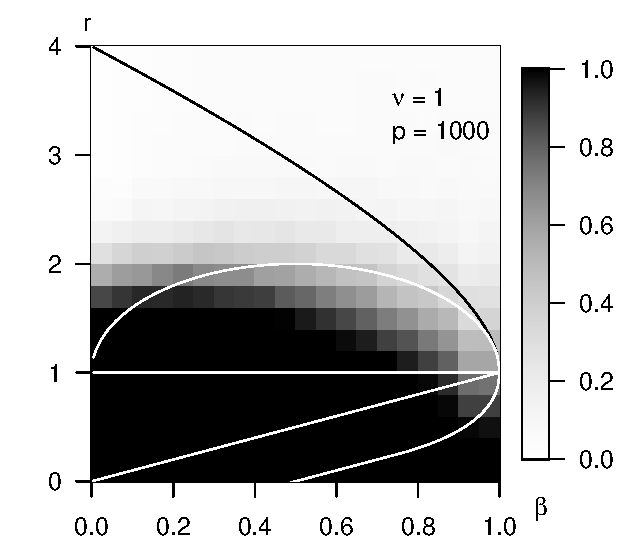
\includegraphics[width=0.32\textwidth]{sim_approx-exact_boundary/simulated_approx-exact_boundary_chi-squared_nu1_p1000.eps}
      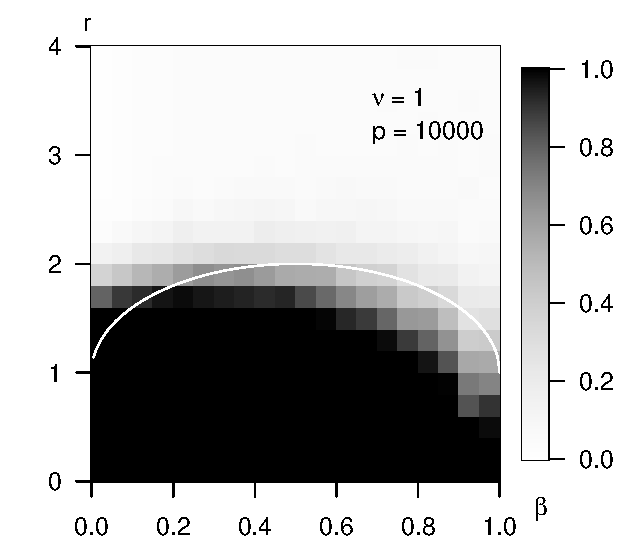
\includegraphics[width=0.32\textwidth]{sim_approx-exact_boundary/simulated_approx-exact_boundary_chi-squared_nu1_p10000.eps}
      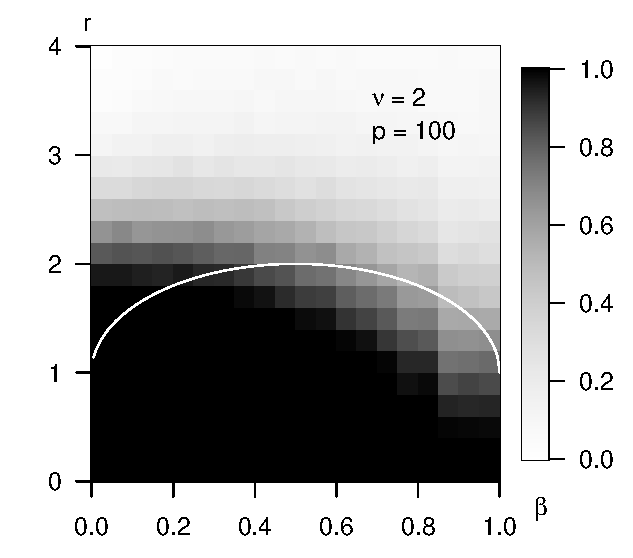
\includegraphics[width=0.32\textwidth]{sim_approx-exact_boundary/simulated_approx-exact_boundary_chi-squared_nu2_p100.eps}
      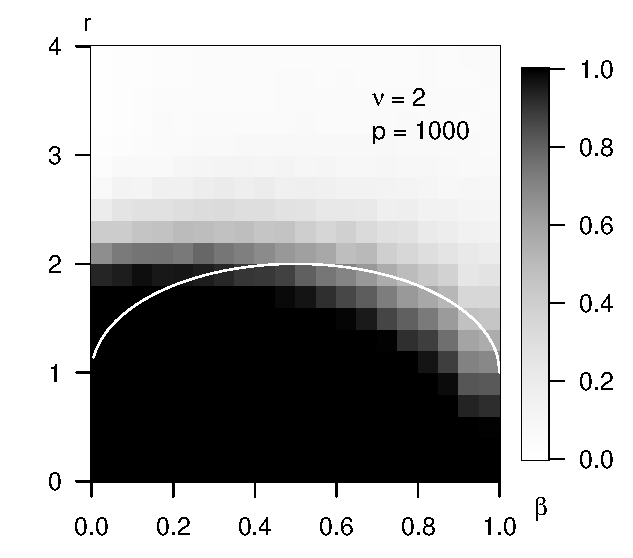
\includegraphics[width=0.32\textwidth]{sim_approx-exact_boundary/simulated_approx-exact_boundary_chi-squared_nu2_p1000.eps}
      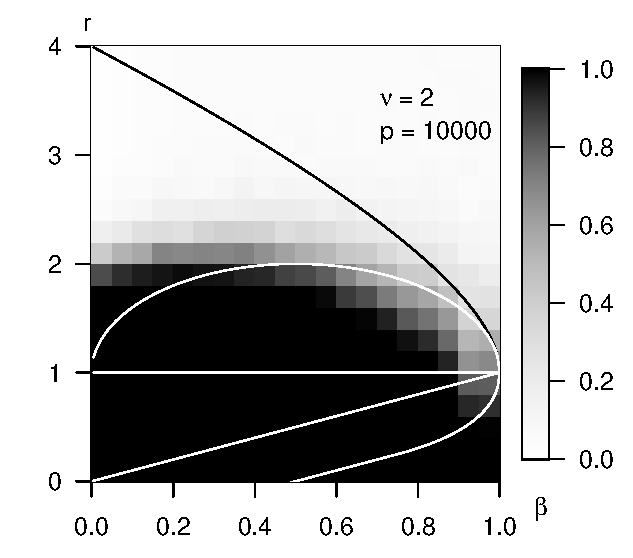
\includegraphics[width=0.32\textwidth]{sim_approx-exact_boundary/simulated_approx-exact_boundary_chi-squared_nu2_p10000.eps}
      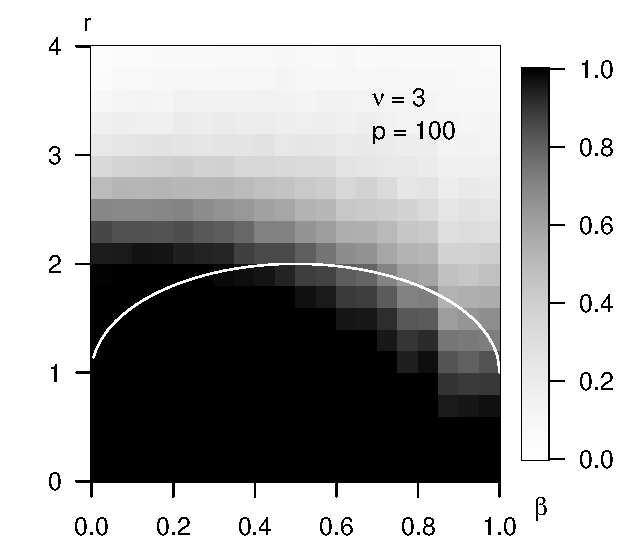
\includegraphics[width=0.32\textwidth]{sim_approx-exact_boundary/simulated_approx-exact_boundary_chi-squared_nu3_p100.eps}
      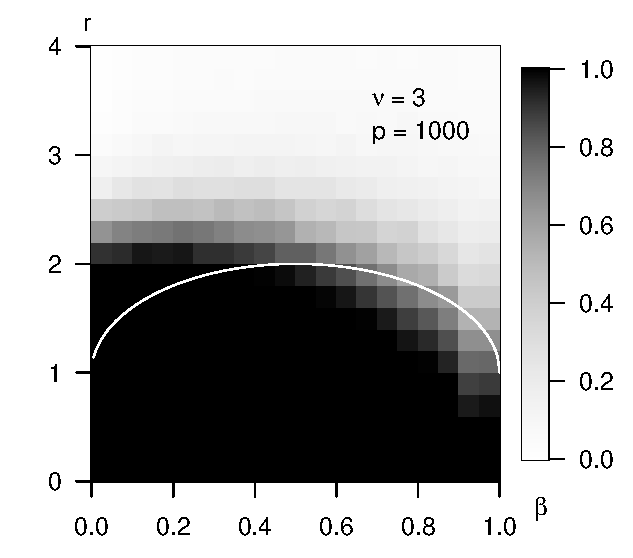
\includegraphics[width=0.32\textwidth]{sim_approx-exact_boundary/simulated_approx-exact_boundary_chi-squared_nu3_p1000.eps}
      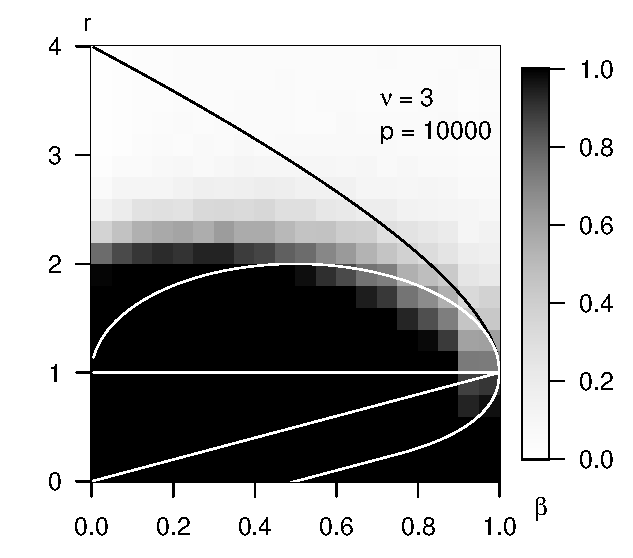
\includegraphics[width=0.32\textwidth]{sim_approx-exact_boundary/simulated_approx-exact_boundary_chi-squared_nu3_p10000.eps}
      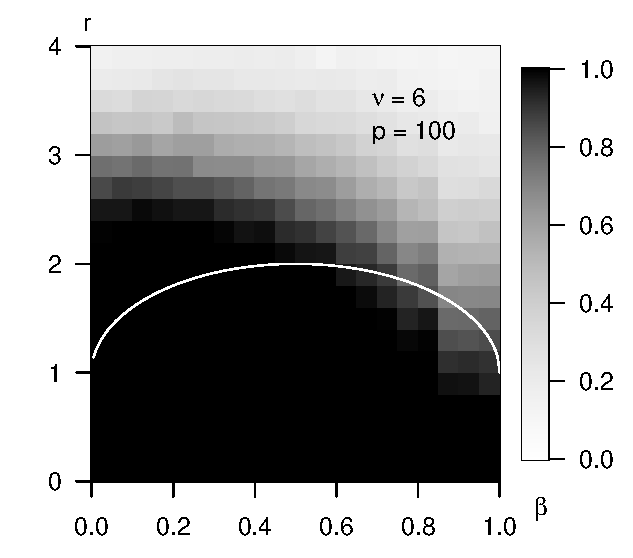
\includegraphics[width=0.32\textwidth]{sim_approx-exact_boundary/simulated_approx-exact_boundary_chi-squared_nu6_p100.eps}
      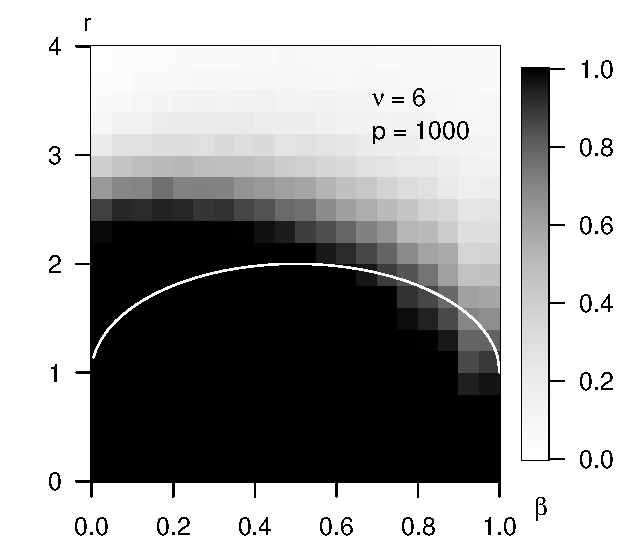
\includegraphics[width=0.32\textwidth]{sim_approx-exact_boundary/simulated_approx-exact_boundary_chi-squared_nu6_p1000.eps}
      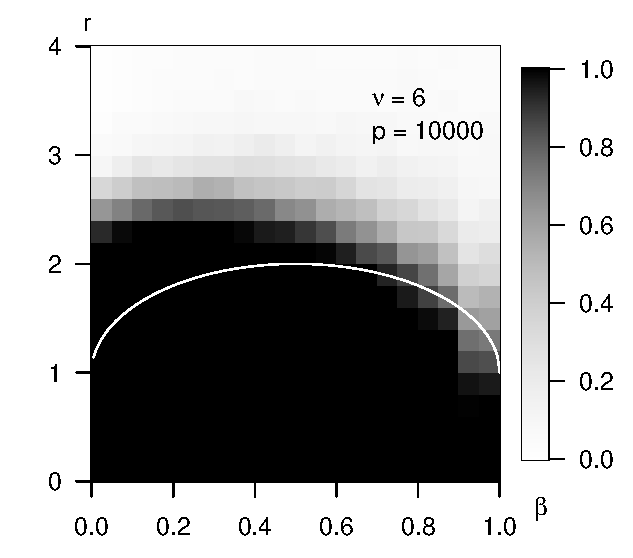
\includegraphics[width=0.32\textwidth]{sim_approx-exact_boundary/simulated_approx-exact_boundary_chi-squared_nu6_p10000.eps}
      \caption{The estimated risk of approximate-exact support recovery $\mathrm{risk}^{\mathrm{EA}}$ (see \eqref{eq:risk-approx-exact}) of the Benjamini-Hochberg procedure in the chi-squared model \eqref{eq:model-chisq}. 
      We simulate $\nu=1, 2, 3, 6$ (first to last row), at dimensions $p=10^2, 10^3, 10^4$ (left to right column), for a grid of sparsity levels $\beta$ and signal sizes $r$.
      The experiments were repeated 1000 times for each sparsity-signal size combination; darker color indicates higher larger $\mathrm{risk}^{\mathrm{EA}}$. 
      Numerical results are generally in agreement with the boundaries described in Theorem \ref{thm:chi-squared-approx-exact-boundary}; for small $\beta$'s and large $\nu$'s, the phase transitions take place somewhat above the predicted boundaries.
      Other boundaries in the support recovery and the detection problems are plotted for comparison.} 
      \label{fig:phase-simulated-chi-squared-approx-exact-boundary}
\end{figure}




\section{Proofs}
\label{sec:proof-signal-size-odds-ratio}

We review some properties of the chi-square distributions in Section \ref{sec:chi-square-distributions}, before presenting the proofs of the main theorems on phase transitions in Sections \ref{subsec:proof-chi-squared-exact-boundary}, \ref{subsec:proof-chi-squared-approx-boundary}, and \ref{subsec:proof-chi-squared-mix-boundaries}.
%Results relating signal sizes and effect sizes in association tests will be justified in Section \ref{subsec:proof-signal-size-odds-ratio}.


\section{Auxiliary facts of chi-square distributions}
\label{sec:chi-square-distributions}
We shall recall, and establish, some auxiliary facts about chi-square distributions. 
These facts will be used in the proofs of Theorem \ref{thm:chi-squared-exact-boundary} and Theorem \ref{thm:chi-squared-approx-boundary}.

\begin{lemma}[Rapid variation of chi-square distribution tails] \label{lemma:rapid-variation-chisq}
The central chi-square distribution with $\nu$ degrees of freedom has rapidly varying tails.
That is, 
\begin{equation} \label{eq:rapid-variation-chisq}
    \lim_{x\to\infty}\frac{\P[\chi_\nu^2(0)>tx]}{\P[\chi_\nu^2(0)>x]} = 
    \begin{cases}
    0, & t > 1 \\
    1, & t = 1 \\
    \infty, & 0 < t < 1
\end{cases},
\end{equation}
where we overloaded the notation $\chi_\nu^2(0)$ to represent a random variable with the chi-square distribution.
\end{lemma}

\begin{proof}[Proof of Lemma \ref{lemma:rapid-variation-chisq}]
When $\nu=1$, the chi-square distribution reduces to a squared Normal, and \eqref{eq:rapid-variation-chisq} follows from the rapid variation of the standard Normal distribution.
For $\nu\ge2$, we recall the following bound on tail probabilities (see, e.g., \citep{inglot2010inequalities}),
$$
\frac{1}{2}\mathcal{E}_\nu(x) \le \P[\chi_\nu^2(0)>x] \le \frac{x}{(x-\nu+2)\sqrt{\pi}} \mathcal{E}_\nu(x), \quad \nu\ge2,\;x>\nu-2,
$$
where $\mathcal{E}_\nu(x) = \exp\left\{-\frac{1}{2}[(x-\nu-(\nu-2)\log(x/\nu) + \log\nu]\right\}$.
Therefore, we have 
$$
\frac{(x-\nu+2)\sqrt{\pi}}{2x}\frac{\mathcal{E}_\nu(tx)}{\mathcal{E}_\nu(x)} 
\le \frac{\P[\chi_\nu^2(0)>tx]}{\P[\chi_\nu^2(0)>x]}
\le \frac{2tx}{(tx-\nu+2)\sqrt{\pi}}\frac{\mathcal{E}_\nu(tx)}{\mathcal{E}_\nu(x)},
$$
where ${\mathcal{E}_\nu(tx)}/{\mathcal{E}_\nu(x)} = \exp\{-\frac{1}{2}[(t-1)x-(\nu-2)\log{t}]\}$ converges to $0$ or $\infty$ depending on whether $t>1$ or $0<t<1$.
The case where $t=1$ is trivial.
\end{proof}

Lemma \ref{lemma:rapid-variation-chisq} and Proposition \ref{prop:rapid-varying-tails} yield the following Corollary.

\begin{corollary} \label{cor:relative-stability}
Maxima of independent observations from central chi-square distributions with $\nu$ degrees of freedom are relatively stable. 
Specifically, let $\epsilon_p = \left(\epsilon_p(i)\right)_{i=1}^p$ be independently and identically distributed (iid) $\chi_\nu^2(0)$ random variables. 
Then the triangular array ${\cal E} = \{\epsilon_p, p\in\N\}$ has relatively stable (RS) maxima in the sense of \eqref{eq:RS-condition}.
\end{corollary}


\begin{lemma}[Stochastic monotonicity] \label{lemma:stochastic-monotonicity}
The non-central chi-square distribution is stochastically monotone in its non-centrality parameter.
Specifically, for two non-central chi-square distributions both with $\nu$ degrees of freedom, and non-centrality parameters $\lambda_1 \le \lambda_2$, we have $\chi^2_\nu(\lambda_1) \stackrel{\mathrm{d}}{\le} \chi^2_\nu(\lambda_2)$. 
That is,
\begin{equation} \label{eq:stochastic-monotonicity}
    \P[\chi^2_\nu(\lambda_1) \le t] \ge \P[\chi^2_\nu(\lambda_2) \le t], \quad \text{for any}\quad t\ge0.
\end{equation}
where we overloaded the notation $\chi_\nu^2(\lambda)$ to represent a random variable with the chi-square distribution with non-centrality parameter $\lambda$ and degree-of-freedom parameter $\nu$.
\end{lemma}

\begin{proof}[Proof of Lemma \ref{lemma:stochastic-monotonicity}]
Recall that non-central chi-square distributions can be written as sums of $\nu-1$ standard normal random variables and a non-central normal random variable with mean $\sqrt{\lambda}$ and variance 1,
\begin{equation*}
    \chi_\nu^2(\lambda) 
    \stackrel{\mathrm{d}}{=} Z_1^2 + \ldots + Z_{\nu-1}^2 + (Z_\nu + \sqrt{\lambda})^2.
\end{equation*}
Therefore, it suffices to show that $\P[(Z+\sqrt{\lambda})^2 \le t]$ is non-increasing in $\lambda$ for any $t\ge0$, where $Z$ is a standard normal random variable.
We rewrite this expression in terms of standard normal probability function $\Phi$,
\begin{align}
    \P[(Z+\sqrt{\lambda})^2 \le t] 
    &= \P[-\sqrt{\lambda} - \sqrt{t} \le Z \le -\sqrt{\lambda} + \sqrt{t}] \nonumber \\
    &= \Phi(-\sqrt{\lambda} + \sqrt{t}) - \Phi(-\sqrt{\lambda} - \sqrt{t}). \label{eq:stochastic-monotonicity-proof-1}
\end{align}
The derivative of the last expression (with respect to $\lambda$) is 
\begin{equation} \label{eq:stochastic-monotonicity-proof-2}
    \frac{1}{2\sqrt{\lambda}} \left(\phi(\sqrt{\lambda} + \sqrt{t}) - \phi(\sqrt{\lambda} - \sqrt{t})\right) 
    = \frac{1}{2\sqrt{\lambda}} \left(\phi(\sqrt{\lambda} + \sqrt{t}) - \phi(\sqrt{t} - \sqrt{\lambda})\right),
\end{equation}
where $\phi$ is the density of the standard normal distribution.
Notice that we have used the symmetry of $\phi$ around 0 in the last expression.

Since $0 \le \max\{\sqrt{\lambda} - \sqrt{t}, \sqrt{t} - \sqrt{\lambda}\} < \sqrt{t} + \sqrt{\lambda}$ when $t>0$, by monotonicity of the normal density on $(0,\infty)$, we conclude that the derivative \eqref{eq:stochastic-monotonicity-proof-2} is indeed negative.
Therefore, \eqref{eq:stochastic-monotonicity-proof-1} is decreasing in $\lambda$, and \eqref{eq:stochastic-monotonicity} follows for $t>0$.
For $t = 0$, equality holds in \eqref{eq:stochastic-monotonicity} with both probabilities being 0.
\end{proof}


Finally, we derive asymptotic expressions for  chi-square quantiles.

\begin{lemma}[Chi-square quantiles] \label{lemma:chisq-quantiles}
Let $F$ be the central chi-square distributions with $\nu$ degrees of freedom, and let $u(y)$ be the $(1-y)$-th generalized quantile of $F$, i.e.,
\begin{equation} \label{eq:quantiles-generic}
    u(y) = F^\leftarrow(1 - y).
\end{equation}
Then 
\begin{equation}
    u(y) \sim 2\log(1/y), \quad \text{as }y\to0. 
\end{equation}
\end{lemma}

\begin{proof}[Proof of Lemma \ref{lemma:chisq-quantiles}]
The case where $\nu=1$ follows from the well-known formula for Normal quantiles (see, e.g., Proposition 1.1 in \cite{gao2018fundamental})
$$
F^\leftarrow(1 - y) = \Phi^\leftarrow(1-y/2)\sim\sqrt{2\log{(2/y)}}\sim\sqrt{2\log{(1/y)}}.
$$
The case where $\nu\ge2$ follows from the following estimates of high quantiles of chi-square distributions (see, e.g., \citep{inglot2010inequalities}),
$$
    \nu +  2\log(1/y) -5/2 \le u(y) \le \nu +  2\log(1/y) + 2\sqrt{\nu\log(1/y)}, \quad \text{for all }y\le0.17,
$$
where both the lower and upper bound are asymptotic to $2\log(1/y)$.
\end{proof}




\section{Proof of Theorem \ref{thm:chi-squared-exact-boundary}}
\label{subsec:proof-chi-squared-exact-boundary}

\begin{proof}[Theorem \ref{thm:chi-squared-exact-boundary}]
We first prove the sufficient condition.
The Bonferroni procedure sets the threshold at $t_p = F^\leftarrow(1-\alpha/p)$, which, by Lemma \ref{lemma:chisq-quantiles}, is asymptotic to $2\log{p} - 2\log{\alpha}$.
By the assumption on $\alpha$ in \eqref{eq:slowly-vanishing-error}, for any $\delta>0$, we have $p^{-\delta}=o(\alpha)$.
Therefore, we have $-\log\alpha\le\delta\log{p}$ for large $p$, and
\begin{equation*} 
    1 \le \limsup_{p\to\infty}\frac{2\log{p} - 2\log{\alpha}}{2\log{p}} \le 1+\delta,
\end{equation*}
for any $\delta>0$.
Hence, $t_p\sim 2\log{p}$.

The condition $\underline{r} > {{g}}(\beta)$ implies, after some algebraic manipulation,
$\sqrt{\underline{r}} -\sqrt{1-\beta} > 1$.
Therefore, we can pick $q>1$ such that 
\begin{equation} \label{eq:choice-of-q}
    \sqrt{\underline{r}} -\sqrt{1-\beta} > \sqrt{q} > 1.
\end{equation}
Setting the $t^* = t^*_p = 2q\log{p}$, we have $t_p < t^*_p$ for large $p$.

On the one hand, $\text{FWER} = 1 - \P[\widehat{S}_p \subseteq S_p]$ vanishes under the Bonferroni procedure with $\alpha\to0$.
On the other hand, for large $p$, the probability of no missed detection is bounded from below by
\begin{equation} \label{eq:chi-square-sufficient-1}
    \P[\widehat{S}_p \supseteq S_p] 
    = \P[\min_{i\in S} x(i) \ge t_p] 
    \ge \P[\min_{i\in S} x(i) \ge t^*] 
    \ge 1 - p^{1-\beta}\P[\chi_\nu^2(\underline{\Delta}) < t^*],
\end{equation}
where we have used the fact that signal sizes are bounded below by $\underline{\Delta}$, and the stochastic monotonicity of chi-square distributions (Lemma \ref{lemma:stochastic-monotonicity}) in the last inequality.
Writing
$$
\chi_\nu^2(\underline{\Delta}) \stackrel{\mathrm{d}}{=} Z_1^2 + \ldots + Z_{\nu-1}^2 + (Z_\nu + \sqrt{\underline{\Delta}})^2
$$
where $Z_i$'s are iid standard normal variables, we have
\begin{align}
    \P[\chi_\nu^2({\underline{\Delta}}) < t^*]
    &\le \P[(Z_\nu+\sqrt{\underline{\Delta}})^2 < t^*] 
    = \P[|Z_\nu+\sqrt{\underline{\Delta}}| < \sqrt{t^*}]  \nonumber \\
    &\le \P\left[Z_\nu < - \sqrt{\underline{\Delta}} +  \sqrt{t^*}\right] \nonumber \\
    &= \P\left[Z_\nu < \sqrt{2\log{p}}\left(\sqrt{q} - \sqrt{\underline{r}}\right)\right]. \label{eq:chi-square-sufficient-2}
\end{align}
By our choice of $q$ in \eqref{eq:choice-of-q}, the last probability in \eqref{eq:chi-square-sufficient-2} can be bounded from above by 
\begin{align*}
    \P\Big[Z_\nu < -\sqrt{2(1-\beta)\log{p}}\Big]
    &\sim \frac{\phi\left(-\sqrt{2(1-\beta)\log{p}}\right)}{\sqrt{2(1-\beta)\log{p}}} \\
    &= \frac{1}{\sqrt{2(1-\beta)\log{p}}}p^{-(1-\beta)},
\end{align*}
where the first line uses Mill's ratio for Gaussian distributions (see Section \ref{sec:Gaussian} and Relation \eqref{eq:Mills-ratio}).
This, combined with \eqref{eq:chi-square-sufficient-1}, completes the proof of the sufficient condition for the Bonferroni's procedure.

Under the assumption of independence, Sid\'ak's, Holm's, and Hochberg's procedures are strictly more powerful than Bonferroni's procedure, while controlling FWER at the nominal levels.
Therefore, the risks of exact support recovery for these procedures also vanishes.
This completes the proof for the first part of Theorem \ref{thm:chi-squared-exact-boundary}.

We now show the necessary condition. 
We first normalize the maxima by the chi-square quantiles $u_p = F^{\leftarrow}(1-1/p)$, where $F$ is the distribution of a (central) chi-square random variable,
\begin{equation} \label{eq:chi-square-necessary-0}
 \P[\widehat{S}_p = S_p] \le \P\left[M_{S^c} <  t_p \le m_{S} \right]
  % &= \P\left[\frac{\max_{i\in S^c}x(i)}{u_p} < \frac{\min_{i\in S}x(i)}{u_p}\right] \nonumber \\
  % &\le  \P\left[\frac{\max_{i\in S^c}\chi_\nu^2(\lambda(i))}{u_p} < \frac{\min_{i\in S}\chi_\nu^2(\lambda(i))}{u_p}\right] \nonumber \\
  \le \P\left[ \frac{M_{S^c}}{u_p} < \frac{m_S}{u_p} \right],
\end{equation}
where $M_{S^c} = \max_{i\in S^c}x(i)$ and $m_{S} = \min_{i\in S}x(i)$.
By the relative stability of chi-square random variables (Corollary \ref{cor:relative-stability}), we know that ${M_{S^c}}/{u_{|S^c|}}\to1$ in probability. 
Further, using the expression for $u_p$ (Lemma \ref{lemma:chisq-quantiles}), we obtain
$$
\frac{u_{p-p^{1-\beta}}}{u_{p}} \sim \frac{2\log{(p-p^{1-\beta})}}{2\log{p}} = \frac{\log{p}+\log{(1-p^{-\beta})}}{\log{p}} \sim 1.
$$
Therefore, the left-hand-side of the last probability in \eqref{eq:chi-square-necessary-0} converges to 1,
\begin{equation} \label{eq:chi-square-necessary-1}
    \frac{M_{S^c}}{u_{p}} = \frac{M_{S^c}}{u_{p-p^{1-\beta}}} \frac{u_{p-p^{1-\beta}}}{u_{p}} \stackrel{\P}{\longrightarrow} 1.
\end{equation}

Meanwhile, for any $i\in S$, by Lemma \ref{lemma:stochastic-monotonicity} and the fact that signal sizes are bounded above by $\overline{\Delta}$, we have,
\begin{equation*}
    {\chi_\nu^2(\lambda(i))} \stackrel{\mathrm{d}}{\le}
    {\chi_\nu^2(\overline{\Delta})} \stackrel{\mathrm{d}}{=} 
    {Z_1^2 + \ldots + Z_{\nu-1}^2 + \left(Z_\nu + \sqrt{\overline{\Delta}}\right)^2}.
\end{equation*}
Dividing through by $u_p$, and taking minimum over $S$, we obtain
\begin{equation} \label{eq:chi-square-necessary-3}
    \frac{m_S}{u_p} 
    = \min_{i\in S} \frac{\chi_\nu^2(\lambda(i))}{u_p} 
    % \stackrel{\mathrm{d}}{\le} \min \left\{\frac{\chi_\nu^2(\overline{\Delta})}{u_p}, s \text{ iid copies} \right\} \\
    \stackrel{\mathrm{d}}{\le} 
    \min_{i\in S}\left\{\frac{Z_1^2(i) + \ldots + Z_{\nu-1}^2(i)}{u_p} + \frac{(Z_\nu(i) + \sqrt{\overline{\Delta}})^2}{u_p}\right\}.
\end{equation}
Let $i^\dagger = i^\dagger_p$ be the index minimizing the second term in \eqref{eq:chi-square-necessary-3}, i.e.,
\begin{equation}
    i^\dagger := \argmin_{i\in S} \frac{(Z_\nu(i) + \sqrt{\overline{\Delta}})^2}{u_p}
    = \argmin_{i\in S} f_p\left(Z_\nu(i)\right),
    % \frac{(Z_\nu(i) + \sqrt{\overline{\Delta}})^2}{2\log{p}},
\end{equation}
where $f_p(x):=(x+\sqrt{\overline{\Delta}})^2/(2\log{p})$. 
We shall first show that 
\begin{equation} \label{eq:chi-square-necessary-4}
    %\min_{i\in S} \frac{(Z_\nu(i) + \sqrt{\overline{\Delta}})^2}{2\log{p}} 
    \P[ f_p(Z_\nu(i^\dagger)) < 1 -\delta ] \to 1,
\end{equation}
for some small $\delta>0$.
On the one hand, we know (by solving a quadratic inequality) that
\begin{equation} \label{eq:chi-square-necessary-5}
    f_p(x)<1-\delta \iff \frac{x}{\sqrt{2\log{p}}} \in (-(\sqrt{\overline{r}}+\sqrt{1-\delta}), -(\sqrt{\overline{r}}-\sqrt{1-\delta})).
\end{equation}
On the other hand, we know (by the relative stability of iid Gaussians, recall Section \ref{sec:Gaussian}) that 
\begin{equation} \label{eq:chi-square-necessary-6}
    % f_p(\min_{i\in S}z_\nu(i)) =
    \frac{\min_{i\in S} Z_\nu(i)}{\sqrt{2\log{p}}}
    \to -\sqrt{1-\beta} \quad\text{in probability}.
\end{equation}
Further, by the assumption on the signal sizes $\overline{r} < (1+\sqrt{1-\beta})^2$, we have,
\begin{equation*}
    -(\sqrt{\overline{r}}+1) < -1 <- \sqrt{1-\beta} < - (\sqrt{\overline{r}}-1).
\end{equation*}
Therefore we can picking a small $\delta>0$ such that 
\begin{equation} \label{eq:chi-square-necessary-7}
    -(\sqrt{\overline{r}}+1) < -(\sqrt{\overline{r}}+\sqrt{1-\delta})
    < - \sqrt{1-\beta}
    < - (\sqrt{\overline{r}}-\sqrt{1-\delta})
    < - (\sqrt{\overline{r}}-1).
\end{equation}
Combining \eqref{eq:chi-square-necessary-5}, \eqref{eq:chi-square-necessary-6}, and \eqref{eq:chi-square-necessary-7}, we obtain
\begin{align*}
    \P\left[\min_{i\in S} f_p(Z_\nu(i)) < 1-\delta\right]
    &= \P\left[ f_p(Z_\nu(i^\dagger)) < 1-\delta \right] \\
    &\ge \P\left[ f_p\left(\min_{i\in S}Z_\nu(i)\right) < 1-\delta \right] \to 1,
\end{align*}
and we arrive at \eqref{eq:chi-square-necessary-4}.
As a corollary, since $u_p\sim2\log{p}$, it follows that
\begin{equation} \label{eq:chi-square-necessary-8}
    \P\left[\min_{i\in S}\frac{(Z_\nu(i) + \sqrt{\overline{\Delta}})^2}{u_p} < 1-\delta\right]\to1.
\end{equation}

Finally, by independence between $Z_1^2(i)+\ldots+Z_{\nu-1}^2(i)$ and $(Z_\nu^2(i)+\sqrt{\overline{\Delta}})^2$, and the fact that $i^\dagger$ is a function of only the latter, we have
$$
Z_1^2(i^\dagger)+\ldots+Z_{\nu-1}^2(i^\dagger) 
\stackrel{\mathrm{d}}{=} Z_1^2(i)+\ldots+Z_{\nu-1}^2(i) 
\quad \text{for all} \;\; i\in S.
$$
Therefore, $Z_1^2(i^\dagger)+\ldots+Z_{\nu-1}^2(i^\dagger) = O_\P(1)$, and 
\begin{equation} \label{eq:chi-square-necessary-9}
    \frac{Z_1^2(i^\dagger)+\ldots+Z_{\nu-1}^2(i^\dagger)}{u_p} \to 0 \quad \text{in probability}. 
\end{equation}
Together, \eqref{eq:chi-square-necessary-8} and \eqref{eq:chi-square-necessary-9} imply that
\begin{align}
    \P\left[\frac{m_S}{u_p}<1-\delta\right]
    &\ge \P\left[\min_{i\in S}\left\{\frac{Z_1^2(i) + \ldots + Z_{\nu-1}^2(i)}{u_p} + \frac{(Z_\nu(i) + \sqrt{\overline{\Delta}})^2}{u_p}\right\} < 1-\delta\right] \nonumber \\
    &\ge \P\left[\frac{Z_1^2(i^\dagger) + \ldots + Z_{\nu-1}^2(i^\dagger)}{u_p} + \frac{(Z_\nu(i^\dagger) + \sqrt{\overline{\Delta}})^2}{u_p} < 1-\delta\right] \to 1. \label{eq:chi-square-necessary-10}
\end{align}
In view of \eqref{eq:chi-square-necessary-0}, \eqref{eq:chi-square-necessary-1}, and \eqref{eq:chi-square-necessary-10}, we conclude that exact recovery cannot succeed with any positive probability.
The proof of the necessary condition is complete.
\end{proof}

\section{Proof of Theorem \ref{thm:chi-squared-approx-boundary}}
\label{subsec:proof-chi-squared-approx-boundary}

We first show the necessary condition. 
That is, when $\overline{r} < \beta$, no thresholding procedure is able to achieve approximate support recovery.

The proof follows the ideas in \cite{arias2017distribution}, and is very similar to the proof of Theorem \ref{thm:Gaussian-error-approx-boundary}. 
One could in principle obtain the proofs in this section by referencing arguments that have appeared in Chapter \ref{chap:phase-transitions}.
We choose to present the proof here in full to make this section self-contained.

\begin{proof}[Necessary condition in Theorem \ref{thm:chi-squared-approx-boundary}]
Denote the distributions of $\chi^2_\nu(0)$, $\chi^2_\nu(\underline{\Delta})$ and $\chi^2_\nu(\overline{\Delta})$ as $F_0$, $F_{\underline{a}}$, and $F_{\overline{a}}$ respectively.

% We first show the necessary condition, i.e., when $\overline{r}<\beta$, approximate support recovery cannot be achieved with any thresholding procedure.
% In particular, we show that the liminf of the sum of FDP and NDP is at least 1.

Recall that thresholding procedures are of the form
$$
\widehat{S}_p = \left\{i\,|\,x(i) > t_p(x)\right\}.
$$
Denote $\widehat{S} := \left\{i\,|\,x(i) > t_p(x)\right\}$, and $\widehat{S}(u) := \left\{i\,|\,x(i) > u\right\}$.
For any threshold $u\ge t_p$ we must have $\widehat{S}(u)\subseteq\widehat{S}$, and hence
\begin{equation} \label{eq:approx-boundary-proof-FDP}
    \text{FDP} := \frac{|\widehat{S}\setminus{S}|}{|\widehat{S}|} \ge \frac{|\widehat{S}\setminus{S}|}{|\widehat{S}\cup{S}|} = \frac{|\widehat{S}\setminus{S}|}{|\widehat{S}\setminus{S}| + |S|} \ge
    \frac{|\widehat{S}(u)\setminus{S}|}{|\widehat{S}(u)\setminus{S}| + |S|}.
\end{equation}
On the other hand, for any threshold $u\le t_p$ we must have $\widehat{S}(u)\supseteq\widehat{S}$, and hence
\begin{equation} \label{eq:approx-boundary-proof-NDP}
    \text{NDP} := \frac{|{S}\setminus\widehat{S}|}{|{S}|} \ge 
    \frac{|{S}\setminus\widehat{S}(u)|}{|{S}|}.
\end{equation}
Since either $u\ge t_p$ or  $u\le t_p$ must take place, putting \eqref{eq:approx-boundary-proof-FDP} and \eqref{eq:approx-boundary-proof-NDP} together, we have
\begin{equation} \label{eq:approx-boundary-proof-converse-1}
    \text{FDP} + \text{NDP} 
    \ge \frac{|\widehat{S}(u)\setminus{S}|}{|\widehat{S}(u)\setminus{S}|+|{S}|} \wedge \frac{|{S}\setminus\widehat{S}(u)|}{|{S}|},
\end{equation}
for any $u$.
Therefore it suffices to show that for a suitable choice of $u$, the RHS of \eqref{eq:approx-boundary-proof-converse-1} converges to 1 in probability; the desired conclusion on FDR and FNR follows by the dominated convergence theorem.

Let $t^* = 2q\log{p}$ for some fixed $q$, we obtain an estimate of the tail probability
\begin{align}
    \overline{F_0}(t^*) 
    &= \P[\chi_\nu^2(0) > t^*] 
    = \frac{2^{-\nu/2}}{\Gamma(\nu/2)} \int_{2q\log{p}}^\infty x^{\nu/2-1}e^{-x/2} \mathrm{d}x \nonumber \\
    &\sim \frac{2^{-\nu/2}}{\Gamma(\nu/2)} 2\left(2q\log{p}\right)^{\nu/2-1}p^{-q}. \label{eq:approx-boundary-proof-null-tail-prob}
\end{align}
where $a_p\sim b_p$ is taken to mean $a_p/b_p\to 1$; this tail estimate was also obtained in \cite{donoho2004higher}.
Observe that $|\widehat{S}(t^*)\setminus{S}|$ has distribution $\text{Binom}(p-s, \overline{F_0}(t^*))$ where $s=|S|$, denote $X = X_p := {|\widehat{S}(t^*)\setminus{S}|}/{|S|}$, and we have 
$$
\mu := \E\left[X\right] = \frac{(p-s)\overline{F_0}(t^*)}{s},
\quad \text{and} \quad
\var\left(X\right) = \frac{(p-s)\overline{F_0}(t^*){F_0}(t^*)}{s^2} \le \mu/s.
$$
Therefore for any $M>0$, we have, by Chebyshev's inequality,
\begin{equation}
    \P\left[X < M\right] 
    \le \P\left[\left|X-\mu\right| > \mu - M\right]
    \le \frac{\mu/s}{(\mu-M)^2}
    = \frac{1/(\mu s)}{(1-M/\mu)^2}. \label{eq:approx-boundary-proof-converse-2}
\end{equation}
Now, from the expression of $\overline{F_0}(t^*)$ in \eqref{eq:approx-boundary-proof-null-tail-prob}, we obtain
$$
\mu = (p^\beta - 1)\overline{F_0}(t^*) \sim \frac{2^{1-\nu/2}}{\Gamma(\nu/2)} \left(2q\log{p}\right)^{\nu/2-1}p^{\beta-q}.
$$
Since $\overline{r}<\beta$, we can pick $q$ such that $\overline{r}<q<\beta$. 
In turn, we have $\mu \to\infty$, as $p\to\infty$.
Therefore the last expression in \eqref{eq:approx-boundary-proof-converse-2} converges to 0, and we conclude that $X\to\infty$ in probability, and hence
\begin{equation} \label{eq:approx-boundary-proof-converse-3}
\frac{|\widehat{S}(t^*)\setminus{S}|}{|\widehat{S}(t^*)\setminus{S}|+|{S}|} 
= \frac{X}{X+1} \to 1 \quad \text{in probability}.
\end{equation}

On the other hand, we show that with the same choice of $u = t^*$,
\begin{equation} \label{eq:approx-boundary-proof-converse-4}
    \frac{|{S}\setminus\widehat{S}(t^*)|}{|{S}|}\to 1 \quad \text{in probability}.
\end{equation}
By the stochastic monotonicity of chi-square distributions (Lemma \ref{lemma:stochastic-monotonicity}), the probability of missed detection for each signal is lower bounded by $\P[\chi^2_\nu(\lambda_i) \le t^*] \ge F_{\overline{a}}(t^*)$.
Therefore, $|{S}\setminus\widehat{S}(t^*)| \stackrel{\mathrm{d}}{\ge} \text{Binom}(s, {F_{\overline{a}}}(t^*))$, and it suffices to show that ${F_{\overline{a}}}(t^*)$ converges to 1.
This is indeed the case, since
\begin{align*}
    {F_{\overline{a}}}(t^*) 
    &= \P[Z_1^2 + \ldots + Z_\nu^2 + 2\sqrt{2\overline{r}\log{p}} Z_\nu + 2\overline{r}\log{p} \le 2q\log{p}] \\
    &\ge \P[Z_1^2 + \ldots + Z_\nu^2 \le (q-\overline{r})\log{p}, \; 2\sqrt{2\overline{r}\log{p}} Z_\nu \le (q-\overline{r})\log{p}],
\end{align*}
and both events in the last line have probability going to 1 as $p\to\infty$.
The necessary condition is shown.
\end{proof}

We now turn to the sufficient condition. 
That is, when $\underline{r} > \beta$, the Benjamini-Hochberg procedure with slowly vanishing FDR levels achieves asymptotic approximate support recovery.
The structure for the proof of sufficient condition follows that of Theorem 2 in \cite{arias2017distribution}. 

\begin{proof}[Sufficient condition in Theorem \ref{thm:chi-squared-approx-boundary}]
The FDR vanishes by our choice of $\alpha$ and the FDR-controlling property of the BH procedure.
It only remains to show that FNR also vanishes.

To do so we compare the FNR under the alternative specified in Theorem \ref{thm:chi-squared-approx-boundary} to one with all of the signal sizes equal to $\underline{\Delta}$.
Let $x(i)$ be vectors of independent observations with $p-s$ nulls having $\chi^2_\nu(0)$ distributions, and $s$ signals having $\chi^2_\nu(\underline{\Delta})$ distributions.
By Lemma \ref{lemma:monotonicity-BH-procedure}, it suffices to show that the FNR under the BH procedure in this setting vanishes.

Let $\widehat{G}$ denote the empirical survival function as in \eqref{eq:empirical-tail-distribution}.
Define the empirical survival functions for the null part and signal part
\begin{equation} \label{eq:empirical-survival-null-signal}
    \widehat{W}_\text{null}(t) = \frac{1}{p-s}\sum_{i\not\in S}\mathbbm{1}\{x(i) \ge t\},
    \quad
    \widehat{W}_\text{signal}(t) = \frac{1}{s}\sum_{i\in S}\mathbbm{1}\{x(i) \ge t\},
\end{equation}
where $s=|S|$, so that
$$
\widehat{G}(t) = \frac{p-s}{p}\widehat{W}_\text{null}(t) + \frac{s}{p}\widehat{W}_\text{signal}(t).
$$


Apply Lemma \ref{lemma:empirical-process} to the two summands in $\widehat{G}$, we obtain
$\widehat{G}(t) = G(t) + \widehat{R}(t)$.
where 
\begin{equation} \label{eq:empirical-process-mean}
    G(t) = \frac{p-s}{p}\overline{F_0}(t) + \frac{s}{p}\overline{F_a}(t),
\end{equation}
where $\overline{F_0}$ and $\overline{F_{a}}$ are the survival functions of $\chi_\nu^2(0)$ and $\chi_\nu^2(\underline{\Delta})$ respectively, and 
\begin{equation} \label{eq:empirical-process-residual}
    \widehat{R}(t) = O_\P\left(\xi_p\sqrt{\overline{F_0}(t)F_0(t)} + \frac{s}{p}\xi_s\sqrt{\overline{F_a}(t)F_a(t)}\right),
\end{equation}
uniformly in $t$.

Recall (see proof of Lemma \ref{lemma:monotonicity-BH-procedure}) that the BH procedure is the thresholding procedure with threshold set at $\tau$ (defined in \eqref{eq:approx-boundary-proof-tau}).
% \begin{equation} \label{eq:approx-boundary-proof-tau-recall}
%     \tau = \inf\{t\,|\,\overline{F_0}(t)\le\alpha\widehat{G}(t)\}. 
%     %= \min\{t\,|\,\overline{F_0}(t)=\alpha\widehat{G}(t)\}.
% \end{equation}
The NDP may also be re-written as 
$$
\text{NDP} = \frac{|{S}\setminus\widehat{S}|}{|{S}|} = \frac{1}{s}\sum_{i\in S}\mathbbm{1}\{x(i) < \tau\} = 1 - \widehat{W}_\text{signal}(\tau),
$$
so that it suffices to show that 
\begin{equation} \label{eq:approx-boundary-proof-sufficient-1}
    \widehat{W}_\text{signal}(\tau)\to 1
\end{equation} in probability.
Applying Lemma \ref{lemma:empirical-process} to $\widehat{W}_\text{signal}$, we know that 
$$
\widehat{W}_\text{signal}(\tau) = \overline{F_a}(\tau) + O_\P\left(\xi_s\sqrt{\overline{F_a}(\tau)F_a(\tau)}\right) = \overline{F_a}(\tau) + o_\P(1).
$$
So it suffices to show that $F_a(\tau)\to 0$ in probability.
Now let $t^* = 2q\log(p)$ for some $q$ such that $\beta<q<\underline{r}$.
We have 
\begin{align}
    F_a(t^*) 
    &= \P[\chi^2_\nu(\underline{\Delta}) \le t^*]
    \le \P\left[2\sqrt{\underline{\Delta}}Z_\nu \le t^* - \underline{\Delta}\right] \nonumber \\
    &= \P\left[Z_\nu \le \frac{t^*}{2\sqrt{\underline{\Delta}}} - \frac{\sqrt{\underline{\Delta}}}{2}\right] 
    = \P\left[Z_\nu \le \frac{q-\underline{r}}{2\sqrt{\underline{r}}}\sqrt{2\log{p}}\right] \to 0. \label{eq:approx-boundary-proof-sufficient-2}
\end{align} 
Hence in order to show \eqref{eq:approx-boundary-proof-sufficient-1}, it suffices to show 
\begin{equation} \label{eq:approx-boundary-proof-sufficient-3}
    \P\left[\tau \le t^*\right] \to 1.
\end{equation}
By \eqref{eq:empirical-process-mean}, the mean of the empirical process $\widehat{G}$ evaluated at $t^*$ is
\begin{equation} \label{eq:approx-boundary-proof-sufficient-4}
    G(t^*) = \frac{p-s}{p}\overline{F_0}(t^*) + \frac{s}{p}\overline{F_a}(t^*).
\end{equation}
The first term, using Relation \eqref{eq:approx-boundary-proof-null-tail-prob}, is asymptotic to $p^{-q}L(p)$, where $L(p)$ is the logarithmic term in $p$.
The second term, since $\overline{F_a}(t^*)\to 1$ by Relation \eqref{eq:approx-boundary-proof-sufficient-2}, is asymptotic to $p^{-\beta}$.
Therefore, $G(t^*) \sim p^{-q}L(p) + p^{-\beta} \sim p^{-\beta}$, since 
$p^{\beta-q}L(p)\to0$ where $q>\beta$.

The fluctuation of the empirical process at $t^*$, by Relation \eqref{eq:empirical-process-residual}, is 
\begin{align*}
    \widehat{R}(t^*) 
    &= O_\P\left(\xi_p\sqrt{\overline{F_0}(t^*)F_0(t^*)} + \frac{s}{p}\xi_s\sqrt{\overline{F_a}(t^*)F_a(t^*)}\right)\\
    &= O_\P\left(\xi_p\sqrt{\overline{F_0}(t^*)}\right) + o_\P\left(p^{-\beta}\right).
\end{align*}
By \eqref{eq:approx-boundary-proof-null-tail-prob} and the expression for $\xi_p$, the first term is $O_\P\left(p^{-(q+1)/2}L(p)\right)$ where $L(p)$ is a poly-logarithmic term in $p$.
Since $\beta<\min\{q,1\}$, we have $\beta<(q+1)/2$, and hence $\widehat{R}(t^*) = o_\P(p^{-\beta})$.

Putting the mean and the fluctuation of $\widehat{G}(t^*)$ together, we obtain
$$
\widehat{G}(t^*) = G(t^*) + \widehat{R}(t^*) \sim_\P G(t^*) \sim p^{-\beta},
$$
and therefore, together with \eqref{eq:approx-boundary-proof-null-tail-prob}, we have
$$
\overline{F_0}(t^*)/\widehat{G}(t^*) = p^{\beta-q}L(p)(1+o_{\P}(1)),
$$
which is eventually smaller than the FDR level $\alpha$ by the assumption \eqref{eq:slowly-vanishing-error} and the fact that $\beta<q$.
That is, 
$$
\P\left[\overline{F}_0(t^*) / \widehat{G}(t^*) < \alpha\right] \to 1.
$$
By definition of $\tau$ (recall \eqref{eq:approx-boundary-proof-tau}), this implies that $\tau \le t^*$ with probability tending to 1, and \eqref{eq:approx-boundary-proof-sufficient-3} is shown.
The proof for the sufficient condition is complete.
\end{proof}

\section{Proof of Theorems \ref{thm:chi-squared-exact-approx-boundary} and \ref{thm:chi-squared-approx-exact-boundary}}
\label{subsec:proof-chi-squared-mix-boundaries}

As with the proof of Theorem \ref{thm:chi-squared-approx-boundary}, one could shorten the presentations in this section by 
referencing arguments in Chapter \ref{chap:phase-transitions}.  Again, we choose to present the proof in full to make this section 
self-contained.

\begin{proof}[Theorem \ref{thm:chi-squared-exact-approx-boundary}]
% The reduction to equal signal sizes can be achieved 
We first show the sufficient condition.
Similar to the proof of Theorem \ref{thm:chi-squared-approx-boundary}, it suffices to show that
\begin{equation} \label{eq:exact-approx-boundary-proof-sufficient-1}
    \text{NDP} = 1 - \widehat{W}_\text{signal}(t_p) \to 0,
\end{equation}
where $t_p$ is the threshold of Bonferroni's procedure.

Since $\underline{r}>\widetilde{g}(\beta)=1$, we can pick $q$ such that $1<q<\underline{r}$.
Let $t^* = 2q\log{p}$, we have $t_p<t_p^*$ for large $p$ as in the proof of Theorem \ref{thm:chi-squared-exact-boundary}.
Therefore for large $p$, we have
$$
\widehat{W}_\text{signal}(t_p) \ge \widehat{W}_\text{signal}(t^*) \ge \overline{F_a}(t^*) + o_\P(1),
$$
where the last inequality follows from the stochastic monotonicity of the chi-square family (Lemma \ref{lemma:stochastic-monotonicity}), and Lemma \ref{lemma:empirical-process}.
Indeed, $F_a(t^*)\to0$ by \eqref{eq:approx-boundary-proof-sufficient-2} and our choice of $q<\underline{r}$. 
The proof of the sufficient condition is complete.

Proof of the necessary condition follows a similar structure to that of Theorem \ref{thm:chi-squared-approx-boundary}.
That is, we show that $\mathrm{FWER} + \mathrm{FNR}$ has liminf at least 1 by working with the lower bound
\begin{equation} \label{eq:exact-approx-boundary-proof-necessary-1}
    \mathrm{FWER}(\mathcal{R}) + \mathrm{FNR}(\mathcal{R}) \ge \P\left[\max_{i\in S^c}x(i)>u\right] \wedge \E\left[\frac{|S\setminus \widehat{S}(u)|}{|S|}\right],
\end{equation}
which holds for any thresholding procedure $\mathcal{R}$ and for arbitrary $u\in\R$.
By the assumption that $\overline{r}<\widetilde{g}(\beta)=1$, we can pick $q$ such that $\overline{r}<q<1$ and let $u = t^*=2q\log{p}$.
By relative stability of chi-squared random variables (Lemma \ref{lemma:rapid-variation-chisq}), we have
\begin{equation} \label{eq:exact-approx-boundary-proof-necessary-2}
    \P\left[\frac{\max_{i\in S^c} x(i)}{2\log{p}} > \frac{t^*}{2\log{p}}\right] \to 1.
\end{equation}
where the first fraction in \eqref{eq:exact-approx-boundary-proof-necessary-2} converges to 1, while the second converges to $q<1$.
On the other hand, by our choice of $q>\overline{r}$, the second term in \eqref{eq:exact-approx-boundary-proof-necessary-1} also converges to 1 as in \eqref{eq:approx-boundary-proof-converse-4}.
This completes the proof of the necessary condition.
\end{proof}


\begin{proof}[Theorem \ref{thm:chi-squared-approx-exact-boundary}]
We first show the sufficient condition.
Since FDR control is guaranteed by the BH procedure, we only need to show that the FWNR also vanishes, that is,
\begin{equation} \label{eq:approx-exact-boundary-proof-sufficient-1}
    \P\left[\min_{i\in S}x(i) \ge \tau\right] \to 1,
\end{equation}
where $\tau$ is the threshold for the BH procedure.

By the assumption that $\underline{r}>\widetilde{h}(\beta)=(\sqrt{\beta}+\sqrt{1-\beta})^2$, we have $\sqrt{\underline{r}}-\sqrt{1-\beta}>\sqrt{\beta}$, so we can pick $q>0$, such that 
\begin{equation} \label{eq:approx-exact-boundary-proof-sufficient-2}
\sqrt{\underline{r}}-\sqrt{1-\beta}>\sqrt{q}>\sqrt{\beta}.
\end{equation}
Let $t^*=2q\log{p}$, we claim that 
\begin{equation} \label{eq:approx-exact-boundary-proof-sufficient-3}
\P\left[\tau\le t^*\right]\to 1.
\end{equation}
Indeed, by our choice of $q>\beta$, \eqref{eq:approx-exact-boundary-proof-sufficient-3} follows in the same way that \eqref{eq:approx-boundary-proof-sufficient-3} did.

With this $t^*$, we have
\begin{equation} \label{eq:approx-exact-boundary-proof-sufficient-4}
    \P\left[\min_{i\in S}x(i) \ge \tau\right] \ge 
    % \P\left[\min_{i\in S}x(i) \ge t^* \ge \tau\right] \ge
    \P\left[\min_{i\in S}x(i) \ge t^*,\; t^* \ge \tau\right].
\end{equation}
However, by our choice of $\sqrt{q} < \sqrt{\underline{r}}-\sqrt{1-\beta}$, the probability of the first event on the right-hand side of \eqref{eq:approx-exact-boundary-proof-sufficient-4} also goes to 1 according to \eqref{eq:chi-square-sufficient-1} and \eqref{eq:chi-square-sufficient-2}.
Together with \eqref{eq:approx-exact-boundary-proof-sufficient-3}, this proves \eqref{eq:approx-exact-boundary-proof-sufficient-1}, and completes proof of the sufficient condition.

The necessary condition follows from the lower bound
\begin{equation} \label{eq:approx-exact-boundary-proof-necessary-1}
    \mathrm{FDR}(\mathcal{R}) + \mathrm{FWNR}(\mathcal{R}) \ge \E\left[\frac{|\widehat{S}(u)\setminus S|}{|\widehat{S}(u)\setminus S| + |S|}\right] \wedge 
    \P\left[\min_{i\in S}x(i)<u\right],
\end{equation}
which holds for any thresholding procedure $\mathcal{R}$ and for arbitrary $u\in\R$.

By the assumption that $\overline{r}<\widetilde{h}(\beta)=(\sqrt{\beta}+\sqrt{1-\beta})^2$, we can pick a constant $q>0$, such that 
\begin{equation} \label{eq:approx-exact-boundary-proof-necessary-2}
    \sqrt{\overline{r}} - \sqrt{1-\beta} < \sqrt{q} < \sqrt{\beta}.
\end{equation}
Let also $u = t^*=2q\log{p}$.
By our choice of $q < \beta$, we know from \eqref{eq:approx-boundary-proof-converse-3} that the first term on the right-hand-side of \eqref{eq:approx-exact-boundary-proof-necessary-1} converges to 1.
It remains to show that the second term in \eqref{eq:approx-exact-boundary-proof-necessary-1} also converges to 1.

For the second term in \eqref{eq:approx-exact-boundary-proof-necessary-1}, dividing through by $2\log{p}$, we obtain
\begin{equation} \label{eq:approx-exact-boundary-proof-necessary-3}
    \P\left[\min_{i\in S}x(i)<t^*\right] = \P\left[ \frac{m_{S}}{2\log{p}} < q \right].
\end{equation}
Similar to \eqref{eq:chi-square-necessary-3}, we have
\begin{equation} \label{eq:approx-exact-boundary-proof-necessary-4}
    \frac{m_{S}}{2\log{p}} 
    \stackrel{\mathrm{d}}{\le} \min_{i\in S}\frac{Z_1^2(i) + \ldots + Z_{\nu-1}^2(i)}{2\log{p}} + \frac{(Z_\nu(i) + \sqrt{\overline{\Delta}})^2}{2\log{p}}.
\end{equation}
Define $i^\dagger = i^\dagger_p$ to be the index minimizing the second term in \eqref{eq:approx-exact-boundary-proof-necessary-4}, i.e.,
\begin{equation}
    i^\dagger := \argmin_{i\in S} f_p\left(Z_\nu(i)\right),
    % \frac{(Z_\nu(i) + \sqrt{\overline{\Delta}})^2}{2\log{p}},
\end{equation}
where $f_p(x):=(x+\sqrt{\overline{\Delta}})^2/(2\log{p})$. 

Since $\sqrt{q}>\sqrt{\overline{r}}-\sqrt{1-\beta}$ and $q>0$, we have
$\frac{\sqrt{\overline{r}}-\sqrt{q}}{\sqrt{1-\beta}}<1$.
Also, since
$$
    \frac{\sqrt{\overline{r}}+\sqrt{q}}{\sqrt{1-\beta}}>0,
    \quad\text{and}\quad
    \frac{\sqrt{\overline{r}}-\sqrt{q}}{\sqrt{1-\beta}} < \frac{\sqrt{\overline{r}}+\sqrt{q}}{\sqrt{1-\beta}},
$$
we can further pick a constant $\beta_0\in(0,1]$ such that
\begin{equation} \label{eq:approx-exact-boundary-proof-necessary-5}
    \frac{\sqrt{\overline{r}}-\sqrt{q}}{\sqrt{1-\beta}} 
    < \sqrt{\beta_0} < 
    \frac{\sqrt{\overline{r}}+\sqrt{q}}{\sqrt{1-\beta}}.
\end{equation}
Let $Z_{[1]}\le Z_{[2]}\le\ldots\le Z_{[s]}$ be the order statistics of 
$\{Z_\nu(i)\}_{i\in S}$ and define $k=\lfloor s^{1-\beta_0}\rfloor$.
Applying Lemma \ref{lemma:relative-stability-order-statistics} (stated below), we obtain
% \begin{equation*} 
% Z_{[k]} \sim -\sqrt{2\beta_0\log{s}} \sim -\sqrt{2\beta_0(1-\beta)\log{p}}.
% % , \quad\text{as}\;\;p\to\infty.
% \end{equation*}
% Therefore, we have,
\begin{equation} \label{eq:approx-exact-boundary-proof-necessary-6}
    % f_p(\min_{i\in S}z_\nu(i)) =
    \frac{Z_{[k]}}{\sqrt{2\log{p}}}
    = \frac{Z_{[k]}}{\sqrt{2\log{s}}} \frac{\sqrt{2\log{s}}}{\sqrt{2\log{p}}} 
    \to -\sqrt{\beta_0(1-\beta)}
    % \left(-(\sqrt{\overline{r}}+\sqrt{q}), -(\sqrt{\overline{r}}-\sqrt{q})\right) 
    \quad\text{in probability}.
\end{equation}
Since we know (by solving a quadratic inequality) that
\begin{equation} \label{eq:approx-exact-boundary-proof-necessary-7}
    f_p(x)<q \iff \frac{x}{\sqrt{2\log{p}}} \in \left(-(\sqrt{\overline{r}}+\sqrt{q}), -(\sqrt{\overline{r}}-\sqrt{q})\right),
\end{equation}
combining \eqref{eq:approx-exact-boundary-proof-necessary-5}, \eqref{eq:approx-exact-boundary-proof-necessary-6}, and 
\eqref{eq:approx-exact-boundary-proof-necessary-7}, it follows that
\begin{equation*}
    %\min_{i\in S} \frac{(Z_\nu(i) + \sqrt{\overline{\Delta}})^2}{2\log{p}} 
    \P\left[ f_p\left(Z_\nu(i^\dagger)\right) < q \right] \ge \P\left[ f_p\left(Z_{[k]}\right) < q \right] \to 1.
\end{equation*}
Finally, using \eqref{eq:chi-square-necessary-9}, we conclude that 
$$
\P\left[\min_{i\in S}x(i)<t^*\right] = 
\P\left[\frac{m_{S}}{2\log{p}} < q\right] \ge
\P\left[o_\P(1) + f_p\left(Z_\nu(i^\dagger)\right) < q \right] \to 1.
$$
Therefore, the two terms on the right-hand-side of \eqref{eq:approx-exact-boundary-proof-necessary-1} both converge 1. 
This completes the proof of the necessary condition.
\end{proof}

It only remains to justify \eqref{eq:approx-exact-boundary-proof-necessary-6}.

\begin{lemma}[Relative stability of order statistics]
\label{lemma:relative-stability-order-statistics}
Let $Z_{[1]} \le \ldots \le Z_{[s]}$ be the order statistics of $s$ iid standard Gaussian random variables.
Let $\beta_0\in(0,1]$ and define $k=\lfloor s^{1-\beta_0}\rfloor$, then we have
\begin{equation}
    \frac{Z_{[k]}}{\sqrt{2\log{s}}} \to -\sqrt{\beta_0} \quad\text{in probability}.
\end{equation}
\end{lemma}

\begin{proof}[Lemma \ref{lemma:relative-stability-order-statistics}]
Using the Renyi representation for order statistics, we write
\begin{equation} \label{eq:relative-stability-order-statistics-proof-1}
    Z_{[i]} = \Phi^{\leftarrow}(U_{[i]}),
\end{equation}
where $U_{[i]}$ is the $i^\mathrm{th}$ (smallest) order statistic of $s$ independent uniform random variables over $(0,1)$.
Since $U_{[i]}$ has a $\mathrm{Beta}(i, s+1-i)$ distribution, with mean and standard deviation,
$$
\E[U_{[k]}] = k/(s+1) \sim s^{-\beta_0}, 
\quad \text{and} \quad
{\mathrm{sd}(U_{[k]})} = \frac{1}{s+1}\sqrt{\frac{k(s+1-k)}{s+2}} \sim s^{-\frac{1+\beta_0}{2}},
$$
we obtain by Chebyshev's inequality 
% (since $\E[U_{[k]}]/\mathrm{sd}(U_{[k]})\sim p^{(1-\beta_0)/2}$) 
$$
\P\left[s^{-\beta_0}(1-\epsilon) < U_{[k]} < s^{-\beta_0}(1+\epsilon)\right] \to 1,
$$
where $\epsilon$ is an arbitrary positive constant.
This implies, by representation \eqref{eq:relative-stability-order-statistics-proof-1},
\begin{equation} \label{eq:relative-stability-order-statistics-proof-2}
    \P\left[\Phi^{\leftarrow}\left(s^{-\beta_0}(1-\epsilon)\right) < Z_{[k]} < \Phi^{\leftarrow}\left(s^{-\beta_0}(1+\epsilon)\right)\right] \to 1.
\end{equation}
Using the expression for standard Gaussian quantiles (see, e.g., Proposition 1.1. in \cite{gao2018fundamental}), we know that
\begin{align*}
    \Phi^{\leftarrow}\left(s^{-\beta_0}(1-\epsilon)\right) 
    &\sim -\sqrt{2\log{\left(s^{\beta_0}/(1-\epsilon)\right)}} \\
    &= -\sqrt{2(\beta_0\log{s} - \log{(1-\epsilon)})} \sim -\sqrt{2\beta_0\log{s}},
\end{align*}
and similarly $\Phi^{\leftarrow}\left(s^{-\beta_0}(1+\epsilon)\right)\sim -\sqrt{2\beta_0\log{s}}$.
Since both ends of the interval in \eqref{eq:relative-stability-order-statistics-proof-2} are asymptotic to $-\sqrt{2\beta_0\log{s}}$, 
% dividing through by $\sqrt{2\log{s}}$, and 
the desired conclusion follows.
\end{proof}




\section{Exercises}
\label{sec:Exercises-GWAS}
\begin{enumerate}
\item

\end{enumerate}
